\documentclass[
  a4paper,            % DIN A4
  DIV=10,             % Schriftgröße und Satzspiegel
  oneside,            % einseitiger Druck
  BCOR=5mm,           % Bindungskorrektur
  parskip=half,       % Halber Abstand zwischen Absätzen
  numbers=noenddot,   % Kein Punkt hinter Kapitelnummern
  bibliography=totoc, % Literaturverzeichnis im Inhaltsverzeichnis
  listof=totoc,       % Abbildungs- und Tabellenverzeichnis im Inhaltsverzeichnis
  %%twoside,            % Doppelseitiges Layout. Auskommentieren für einseitiges Layout
  table
]{scrreprt}
\usepackage{../style/thesisstyle}
\usepackage{float}
\usepackage{booktabs}
\usepackage{array}
\usepackage{placeins}
\usepackage{hyperref}
\usepackage{cleveref}
\usepackage{listings}
\usepackage{xcolor}
\usepackage{graphicx}
\usepackage{microtype}
\usepackage{caption}
\captionsetup{justification=raggedright,singlelinecheck=false}



\makeglossaries           % create all glossary entries (remember: run makeglossaries manually)
\loadglsentries{thesisglossaries.tex}  % load acronym, symbol and glossary entries

\sisetup{locale = DE}     % siunitx locale setup
%\DeclareSIUnit \fps{fps}  % a custom unit (usage: \SI{24}{\fps})

\begin{document}
% !TEX root = ../thesis.tex
%
% configurations
%

% English Language support
% -> uncomment if needed
% Beta!
%\fullenglish{yes}
\fullenglish{no}

% text field
%-> replace supervisor names with correct ones
\firstSupervisor{Prof. Dr.-Ing. Jane Doe}
\secondSupervisor{Prof. Dr. John Doe}

% text field
%-> replace title with your thesis title
\thesisTitle{Das Leben, das Universum und der ganze Rest}
\thesisTitleEN{Life, the Universe and Everything}

% text field
%-> replace the key words with your own key words
\keywordsDE{Leben, Universum, Alles}
\keywordsEN{Life, Universe, Everything}

% text field
%-> replace the text with a description of the thesis
\abstractDE{Arthur Dents Reise in eine neue Zukunft \dots}
\abstractEN{Arthur Dents travel to a new future \dots}

% text field
%-> replace john with your name
\thesisAuthor{John Doe}

% text field
%-> enter the submission date
\submissionDate{07. Juni 1954}

% switch - uncomment only one
%-> uncomment NDA or public
%\NDA{yes}
\NDA{no}

% switch - uncomment only one
%-> uncomment old standard cover or cover Corporate Design 2017
\Cover{CD2017}
%\Cover{CD2017NoLogo}
%\Cover{Std2018}
%\Cover{Std2018_green} 			% with green bar

% switch - uncomment only one
%-> uncomment to show list of figures or not
\ListOfFigures{yes}
%\ListOfFigures{no}

% switch - uncomment only one
%-> uncomment to show list of tables or not
\ListOfTables{yes}
%\ListOfTables{no}

% switch - uncomment only one
%-> uncomment to show list of accronyms or not
\ListOfAccronyms{yes}
%\ListOfAccronyms{no}

% switch - uncomment only one
%-> uncomment to show list of symbols or not
\ListOfSymbols{yes}
%\ListOfSymbols{no}

% switch - uncomment only one
%-> uncomment to show list of glossary entries or not
\Glossary{yes}
%\Glossary{no}

% switch - uncomment only one
%-> uncomment the study course you are in
\studycourse{INF_ITS}   % Informatik Technischer Systeme
%\studycourse{INF_AI}   % Angewandte Informatik
%\studycourse{INF_WI}   % Wirtschaftsinformatik
%\studycourse{INF_ECS}  % European Computer Science
%\studycourse{EMI_EI}   % Elektrotechnik und Informationstechnik
%\studycourse{EMI_REE}  % Regenerative Energiesysteme und Energiemanagement
%\studycourse{EMI_IE}   % Inforamation Engineering
%\studycourse{BMP}      % Mechanical Engineering
%\studycourse{BMP-hp}   % Mechanical Engineering - Internship Report
%\studycourse{BMT}      % Mechatronik
%\studycourse{BMT-st}   % Study / home assignment in BMT
%\studycourse{BMT-hp}   % Internship Report
%\studycourse{INF_MaI}      % Master Informatik
%\studycourse{EMI_MaA}      % Master Automatisierung
%\studycourse{EMI_MaICE}    % Master Information and Communication Engieering
%\studycourse{EMI_MaMS}     % Master Microelectronic Systems
    % load all settings

\hyphenation{Ba-che-lor-the-sis Mas-ter-the-sis}

% Cover page here, no page number
\ICoverPage

% PDF Metadata
\input{../style/metadata}

% Titlepage is page one even if the number is not shown.
\pagenumbering{roman}
% Title page here
\cleardoublepage
\input{../style/titlepage}

% Abstract page here
\cleardoublepage
\input{../style/abstractpage}

% Table of contents here
\cleardoublepage
\tableofcontents

% List of figures here
\cleardoublepage
\IListOfFigures

% List of tables here
\cleardoublepage
\IListOfTables

% List of accronyms here
\cleardoublepage
\IListOfAccronyms

% List of symbols here
\cleardoublepage
\IListOfSymbols

% Uncomment if list of source code is needed (rarely).
%\lstlistoflistings  % requires package listings, needs to uncommenting of usepackage

% path to the chapters folder is set to find the images used there
\graphicspath{ {./chapters/} }

% Chapters
\cleardoublepage
\pagenumbering{arabic}
% first example chapter
% @author Thomas Lehmann (angepasst für Framarz Alizadeh)
%
\chapter{Einleitung}
\label{chap:einleitung}
Die manuelle Rechnungs- und Dokumentenverarbeitung ist insbesondere für kleine Dienstleistungsunternehmen mit erhöhtem Zeitaufwand und einer erhöhten Fehleranfälligkeit verbunden \cite{chatbots_finanzprozesse}. Diese Arbeit entwickelt 
einen Chatbot-basierten Ansatz zur Digitalisierung, der Medienbrüche reduziert 
und administrative Prozesse automatisiert. Zunächst wird die Problemstellung 
skizziert, bevor Motivation, Ziele und Forschungsfragen erläutert werden.

\section{Problemstellung}
\label{sec:problemstellung}

Kleine Dienstleistungsunternehmen und selbstständige Erwerbstätige verfügen häufig über keine spezialisierte Buchhaltungs- oder \gls{ac:erp}-Software, sondern erstellen ihre Rechnungen mit einfachen Office-Werkzeugen wie Textverarbeitungs- oder Tabellenkalkulationsprogrammen \cite{bitkom_kmu_digitalisierung_2023}. Kundendaten, Leistungsbeschreibungen sowie Beträge werden dabei manuell in Vorlagen übertragen. Die Rechnungen werden anschließend als \gls{ac:pdf} exportiert und per E-Mail oder Messenger an die Kundschaft versendet. Die Ablage der erzeugten Rechnungen und weiterer administrativer Dokumente erfolgt oftmals in unsystematischen Ordnerstrukturen auf lokalen Rechnern oder in allgemeinen Cloud-Speichern.

Diese Vorgehensweise führt zu mehreren Problemen. Zum einen ist die wiederkehrende manuelle Erstellung und Ablage von Rechnungen zeitaufwendig und fehleranfällig, etwa durch Tippfehler, fehlende oder unvollständige Pflichtangaben sowie uneinheitliche Formatierungen. Zum anderen entstehen Medienbrüche zwischen Kommunikationskanälen, Office-Dokumenten und Ablagesystemen, da Informationen aus E-Mails, Chats oder Notizen in unterschiedlichen Systemen erneut eingegeben und gepflegt werden müssen. Dies erschwert die spätere Nachvollziehbarkeit von Belegen, die strukturierte Vorbereitung von Unterlagen für Steuerberatung und Finanzverwaltung sowie den schnellen Zugriff auf vergangene Rechnungen und relevante Dokumente \cite{chatbots_finanzprozesse,manual_invoice_time_2025}.

Gleichzeitig stehen einfache cloudbasierte Werkzeuge zur Verfügung, mit denen sich Datenhaltung, Dokumentenerzeugung und Kommunikation grundsätzlich integrieren ließen. Viele kleine Unternehmen nutzen solche Dienste jedoch isoliert und ohne durchgängige Automatisierung, etwa indem sie zwar Cloud-Speicher oder Online-Textverarbeitung einsetzen, die dazwischenliegenden Prozesse aber weiterhin manuell ausführen. Es fehlt eine niedrigschwellige Lösung, die an den alltäglichen Arbeitsgewohnheiten der Zielgruppe ansetzt, Medienbrüche reduziert und sowohl die Erstellung als auch die strukturierte Ablage von Rechnungen und administrativen Dokumenten unterstützt, ohne den Einsatz komplexer und kostenintensiver Buchhaltungssysteme zu erfordern \cite{ifm_kmu_digitalisierung_prozesse}.

\section{Motivation und Zielsetzung}
\label{sec:motivation-zielsetzung}
Die in \autoref{sec:problemstellung} beschriebene Ausgangslage zeigt, dass viele kleine Dienstleistungsunternehmen und Selbstständige zwar grundlegende digitale Werkzeuge nutzen, ihre administrativen Prozesse jedoch weiterhin stark manuell und medienbruchbehaftet organisieren. Rechnungen werden häufig erst mit zeitlichem Abstand zur erbrachten Leistung erstellt, die notwendigen Informationen müssen aus E-Mails, Notizen oder Gesprächen zusammengesucht werden, und die Ablage der entstandenen Dokumente erfolgt ohne konsistente Struktur. Dies führt nicht nur zu vermeidbarem Zeitaufwand und Fehlern, sondern erschwert auch die transparente Vorbereitung von Unterlagen für Steuerberatung und Finanzverwaltung.

Vor diesem Hintergrund besteht die Motivation dieser Arbeit darin, einen niedrigschwelligen Ansatz zur Digitalisierung der Rechnungs- und Dokumentenverarbeitung zu untersuchen, der sich an den realen Arbeitsgewohnheiten der Zielgruppe orientiert. Statt eine weitere, eigenständige Fachanwendung einzuführen, soll ein System entworfen werden, das an einen bereits etablierten Kommunikationskanal anknüpft und administrative Tätigkeiten dialogbasiert unterstützt. Durch die Kombination eines Chatbots mit einer cloudbasierten Datenhaltung und einer ergänzenden Web-Anwendung sollen Medienbrüche reduziert, wiederkehrende Arbeitsschritte automatisiert und eine strukturierte, nachvollziehbare Ablage der entstehenden Dokumente ermöglicht werden.

Ziel der Arbeit ist es, ein prototypisches System zu konzipieren und zu implementieren, das die Erstellung von Rechnungen und die Ablage administrativer Dokumente für kleine Unternehmen und Selbstständige unterstützt. Konkret soll der Prototyp es ermöglichen, Rechnungsdaten dialoggeführt über einen Chatbot zu erfassen, auf Basis eines Templates automatisiert Rechnungsdokumente zu erzeugen und diese in einer konsistenten Struktur in der Cloud abzulegen. Ergänzend soll eine Web-Anwendung Kunden, Rechnungen und Dokumente übersichtlich darstellen und verwalten.

Die Arbeit entstand im Rahmen der Unterstützung eines selbstständigen Schneiders aus Winterhude, der etwa dreimal im Monat Rechnungen erstellen muss. Für ihn als Nicht-Muttersprachler fällt die manuelle Erstellung mit korrekter Formatierung, Pflichtangaben und Ablage besonders schwierig, da die deutsche Fachsprache im Rechnungswesen und die ständige Suche nach Vorlagen und Kundendaten viel Zeit und Frustration verursachen. Das entwickelte System adressiert genau diese praktischen Herausforderungen einer typischen Zielgruppenperson.

Die Umsetzung soll zeigen, inwieweit sich mit verhältnismäßig einfachen, cloudbasierten Bausteinen ein durchgängiger, medienarmer Prozess realisieren lässt und welche Grenzen und Verbesserungspotenziale sich im praktischen Einsatz eines solchen Ansatzes ergeben.

\section{Forschungsfragen}
\label{sec:forschungsfragen}

Aus der in \autoref{sec:problemstellung} beschriebenen Ausgangslage sowie der in \autoref{sec:motivation-zielsetzung} formulierten Zielsetzung ergeben sich die folgenden Forschungsfragen, die im Rahmen dieser Arbeit untersucht werden:

\begin{enumerate}
\item Wie lässt sich ein prototypisches System zur Erstellung und strukturierten Ablage von Rechnungen und administrativen Dokumenten für kleine Dienstleistungsunternehmen und Selbstständige auf Basis gängiger cloudbasierter Werkzeuge konzipieren?
\item Inwieweit kann ein Chatbot, der an einen bestehenden Kommunikationskanal angebunden ist, die dialogbasierte Erfassung von Rechnungs- und Dokumentendaten unterstützen, sodass Medienbrüche reduziert und wiederkehrende manuelle Arbeitsschritte verringert werden?
\item Wie kann eine ergänzende Web-Anwendung gestaltet werden, die einen strukturierten Zugriff auf Kunden, Rechnungen und Dokumente ermöglicht und die im Chat erfassten Daten für die weitere Verwaltung nutzbar macht?
\item Inwieweit zeigen sich beim praktischen Einsatz des prototypisch umgesetzten Systems Grenzen, Herausforderungen und Verbesserungspotenziale in Bezug auf Nutzbarkeit, Prozessdurchlaufzeiten und technische Robustheit?
\end{enumerate}


\section{Vorgehensweise und Aufbau der Arbeit}
\label{sec:vorgehensweise-aufbau}

Die vorliegende Arbeit gliedert sich in mehrere aufeinander aufbauende Schritte, die von der Einordnung des Themas über die Konzeption bis hin zur prototypischen Umsetzung und Evaluation des Systems reichen. Ziel ist es, die in den vorherigen Abschnitten formulierten Forschungsfragen systematisch zu bearbeiten und die dabei getroffenen Entscheidungen nachvollziehbar zu begründen.

Zunächst werden in \autoref{chap:grundlagen} die fachlichen und technischen Grundlagen vorgestellt, die für das Verständnis der Arbeit erforderlich sind. Dazu gehören insbesondere zentrale Konzepte der Rechnungs- und Dokumentenverarbeitung in kleinen Unternehmen sowie relevante Aspekte cloudbasierter Dienste und Integrationsplattformen. Auf dieser Basis werden zudem die in der Arbeit eingesetzten Technologien eingeordnet und begrifflich abgegrenzt.

Im anschließenden Kapitel wird die Konzeption des zu entwickelnden Systems beschrieben. Dabei werden die fachlichen Anforderungen präzisiert, zentrale Use-Cases herausgearbeitet und eine Zielarchitektur entworfen, die den Einsatz eines Chatbots, einer cloudbasierten Datenhaltung und einer ergänzenden Web-Anwendung miteinander verbindet. Die Konzeption umfasst sowohl die Gestaltung der Dialoge im Chat als auch die Struktur der zugrunde liegenden Daten und Dokumente.

Darauf aufbauend folgt die Implementierung des Prototyps. In diesem Kapitel wird erläutert, wie die zuvor konzipierte Architektur mit konkreten Werkzeugen und Diensten umgesetzt wird. Beschrieben werden die technische Integration der einzelnen Komponenten, die wichtigsten Implementierungsentscheidungen sowie ausgewählte Aspekte der praktischen Realisierung.

Im anschließenden Evaluationskapitel wird das entwickelte System anhand ausgewählter Szenarien untersucht. Dabei werden insbesondere die funktionale Vollständigkeit der Kernprozesse, die wahrgenommene Performance aus Nutzersicht sowie die Stärken und Grenzen des Ansatzes im praktischen Einsatz betrachtet. Zudem werden identifizierte Herausforderungen und mögliche Erweiterungen diskutiert.

Abschließend fasst das Schlusskapitel die wesentlichen Ergebnisse der Arbeit zusammen, beantwortet die eingangs formulierten Forschungsfragen und gibt einen Ausblick auf weiterführende Arbeiten sowie potenzielle Weiterentwicklungen des prototypischen Systems.


% first example chapter
% @author Thomas Lehmann
%
\chapter{Theoretische Grundlagen}
\label{chap:grundlagen}
In diesem Kapitel werden die fachlichen und technischen Grundlagen vorgestellt, 
die für das Verständnis der Arbeit erforderlich sind. Zunächst erfolgt eine 
Einführung in die Digitalisierung administrativer Prozesse und spezifische 
Anforderungen im Rechnungswesen kleiner Unternehmen. Anschließend werden 
Chatbots und dialogbasierte Systeme beleuchtet, gefolgt von cloudbasierter Datenhaltung
und Integrationen. Darauf aufbauend folgen Dokumentengenerierung 
in der Cloud sowie Grundlagen moderner Webanwendungen als zentrale Bausteine 
der Lösung.

\section{Digitalisierung administrativer Prozesse und Rechnungswesen}
\label{sec:digitalisierung-rechnungswesen}
Die vorliegende Arbeit richtet sich nicht an Großunternehmen mit etablierten \gls{ac:erp}- und Buchhaltungssystemen. Im Fokus stehen vielmehr kleine Dienstleistungsunternehmen und Einzelunternehmer, die ihre administrativen Aufgaben überwiegend ohne eigene Buchhaltungsabteilung bewältigen. Zu dieser Zielgruppe zählen insbesondere Freelancer sowie Kleinstbetriebe wie Handwerker, Berater, Coaches oder Fotografen. Darüber hinaus werden auch kleine Agenturen und Dienstleistungsbetriebe mit wenigen Mitarbeitenden berücksichtigt. In diesen Unternehmen stützt sich das Rechnungswesen häufig auf einfache Office-Werkzeuge und wenig strukturierte Ablagesysteme \cite{word_excel_kmu_rechnungen,bitkom_elektronische_rechnungsdaten_2022}. Viele administrative Tätigkeiten werden manuell durchgeführt und binden einen erheblichen Teil der verfügbaren Arbeitszeit. Für diese Zielgruppe stellt die Digitalisierung administrativer Prozesse eine zentrale Chance dar. Sie ermöglicht es, den manuellen Aufwand im Tagesgeschäft zu reduzieren und gleichzeitig die Qualität sowie Nachvollziehbarkeit finanzieller Informationen nachhaltig zu verbessern.

Im Alltag nutzen kleine Unternehmen häufig Word- oder Excel-Vorlagen zur Erstellung von Angeboten und Rechnungen. Bestehende Dokumente werden dabei kopiert und manuell angepasst. Kundendaten, Rechnungsnummern, Datumsangaben sowie Beträge und Steuerinformationen müssen wiederholt per Hand eingetragen werden. Dieses Vorgehen ist zeitaufwendig und fehleranfällig. Aufgrund fehlender Systemunterstützung können Tippfehler, unvollständige Angaben oder doppelt vergebene Rechnungsnummern entstehen. Die Kommunikation mit Kunden und Steuerberatungen erfolgt zudem überwiegend per E-Mail, wodurch häufig mehrere Versionen derselben Rechnung im Umlauf sind und zusätzlicher Abstimmungsaufwand entsteht. Belege liegen darüber hinaus in unterschiedlichen Formaten vor, etwa als Papierdokumente, Scans, Smartphone-Fotos oder \gls{ac:pdf}-Anhänge. Die Ablage erfolgt häufig unsystematisch in lokalen Ordnerstrukturen, Cloud-Speichern oder direkt im E-Mail-Postfach. Ein einheitliches Ordnungsprinzip nach Kunden oder Zeiträumen fehlt dabei oftmals. Diese Arbeitsweise ist von zahlreichen Medienbrüchen geprägt, da Informationen manuell zwischen verschiedenen Anwendungen und Dokumenten übertragen werden müssen. Jeder Wechsel zwischen Medien und Systemen erfordert zusätzliche manuelle Eingriffe und erhöht die Fehleranfälligkeit. Gleichzeitig nimmt die Transparenz über den aktuellen Status von Rechnungen und Belegen ab. Insbesondere vor periodischen Stichtagen wie Monats- oder Jahresabschlüssen führt diese Situation zu zusätzlichem organisatorischem Aufwand und erhöhtem Stress, da Unterlagen für Steuerberaterinnen und Steuerberater häufig nachträglich zusammengestellt werden müssen. Verzögerte oder fehlerhafte Rechnungen wirken sich zudem unmittelbar auf die Liquidität aus, da Zahlungseingänge verspätet erfolgen und offene Posten schwerer nachzuvollziehen sind \cite{chatbots_finanzprozesse}.

Die Digitalisierung administrativer Prozesse im Rechnungswesen verfolgt mehrere zentrale Ziele. Ein wesentliches Ziel ist die Verkürzung von Durchlaufzeiten. Wiederkehrende Prozessschritte wie das Erstellen, Versenden und Ablegen von Rechnungen sollen hierzu standardisiert und weitgehend automatisiert ablaufen. Darüber hinaus soll die Nachvollziehbarkeit verbessert werden. Rechnungen und zugehörige Dokumente werden zentral abgelegt und eindeutig Kunden sowie Zeiträumen zugeordnet. Dadurch sind sie jederzeit auswertbar, und die Transparenz über den Status von Belegen und Zahlungsvorgängen wird erhöht. Ein weiterer Schwerpunkt liegt auf der Reduktion redundanter Dateneingaben. Kundendaten, Leistungsbeschreibungen und Zahlungsinformationen sollen nur einmal strukturiert erfasst und anschließend in unterschiedlichen Kontexten wiederverwendet werden. Dazu zählen unter anderem die Rechnungserstellung, Auswertungen und die Vorbereitung für die Steuerberatung. Cloudbasierte Lösungen ermöglichen zudem einen orts- und zeitunabhängigen Zugriff auf Rechnungen und Belege. Dadurch werden sowohl die Zusammenarbeit mit externen Dienstleistern als auch mobile Arbeitsformen erleichtert \cite{chatbots_finanzprozesse, bitkom_elektronische_rechnungsdaten_2022}.

In Bezug auf das Szenario sind vor allem die Informationen entscheidend, die nötig sind, um eine korrekte und nachvollziehbare Rechnungserstellung zu gewährleisten. Hierzu gehören konsistente Kundendaten wie Adresse und Umsatzsteuer-Identifikationsnummer, eindeutige Rechnungsnummern und Rechnungsdaten sowie strukturierte Leistungsbeschreibungen mit Mengen- und Preisangaben. Darüber hinaus sind steuerliche Kenngrößen und klar definierte Zahlungsbedingungen von Bedeutung. Das System, das in dieser Arbeit entworfen wurde, adressiert diese Anforderungen bewusst als Vorstufe zur Finanzbuchhaltung. Es ermöglicht die strukturierte Erfassung von Rechnungsdaten, die zentrale Verwaltung von Kundenstammdaten, die automatisierte Erstellung von Dokumenten und eine revisionssichere Ablage der erzeugten Belege. Es werden weder Hauptbücher geführt noch Buchungssätze erstellt. Aufgaben wie die Kontierung, die Umsatzsteuervoranmeldung oder der Jahresabschluss bleiben nach wie vor bei Steuerberatungen und spezialisierten Buchhaltungssystemen. Sie können auf den konsistenten Beleg- und Stammdaten aufbauen, die das System bereitstellt, und die weiterführende buchhalterische Verarbeitung übernehmen.

Der in dieser Arbeit verfolgte Chatbot-basierte Ansatz unterscheidet sich grundlegend von klassischen, formularorientierten Rechnungsprogrammen, wie sie typischerweise über webbasierte Benutzeroberflächen bereitgestellt werden. Herkömmliche Systeme setzen voraus, dass Nutzer aktiv eine Anwendung öffnen, sich durch Masken und Menüs navigieren und eigenständig entscheiden, welche Felder auszufüllen sind. Der hier vorgestellte Ansatz verfolgt hingegen eine schrittweise, dialogbasierte Datenerfassung über einen bereits etablierten Kommunikationskanal. Nutzer interagieren mit dem System ähnlich wie mit einem Kontakt in einem Messenger und werden im Gesprächsverlauf gezielt durch den Erfassungsprozess geführt. Die selbstständige Bedienung komplexer Formulare ist dadurch nicht erforderlich. Dieser Ansatz senkt insbesondere für technisch weniger affine Anwender die Einstiegshürde. Zudem ermöglicht er eine situative Datenerfassung direkt im Arbeitskontext, etwa unmittelbar nach Abschluss einer Dienstleistung. Geführte Eingaben und integrierte Validierungen tragen zusätzlich dazu bei, die Fehleranfälligkeit zu reduzieren. Studien und Praxisberichte zur Automatisierung von Finanzprozessen, insbesondere bei KMU-Rechnungsprozessen, zeigen dass digitale Systeme insbesondere bei der Verarbeitung von Rechnungs- und Ausgabendaten Effizienzgewinne erzielen und gleichzeitig die Fehlerquote verringern können \cite{chatbots_finanzprozesse}.



\section{Chatbots und dialogbasierte Systeme}
\label{sec:chatbots}
Chatbots sind Softwaresysteme, die mit Nutzenden über natürliche Sprache oder strukturierte Eingaben interagieren und dabei eine Konversation simulieren. Sie werden typischerweise in Messaging-Plattformen, Web-Chats oder Sprachassistenten eingebettet und dienen als Schnittstelle zu dahinterliegenden Informations- und Prozesssystemen. Abhängig von ihrer technischen Ausgestaltung reicht das Spektrum von einfachen, regelbasierten Antwortsystemen bis hin zu KI-basierten Assistenten. Letztere nutzen statistische Sprachmodelle, um Kontext zu berücksichtigen und flexibel auf unterschiedliche Eingaben reagieren zu können \cite{chatbots_grundlagen}.

Früher Chatbots waren überwiegend regelbasiert aufgebaut. Sie arbeiteten mit fest definierten Dialogbäumen, Schlüsselwörtern und statischen Antwortbausteinen. Der Dialogverlauf wurde dabei durch If-Then-Regeln oder Zustandsautomaten gesteuert und konnte nur eine begrenzte Anzahl möglicher Interaktionen abbilden. Moderne dialogbasierte Systeme nutzen hingegen Verfahren der automatischen Sprachverarbeitung. Diese ermöglichen es, Benutzereingaben zu analysieren, Intentionen zu erkennen und relevante Entitäten wie Beträge, Datumsangaben oder Kundennamen zu extrahieren. Auf dieser Grundlage können solche Systeme komplexere Aufgaben übernehmen, etwa das Ausfüllen von Formularen, das Zusammenfassen von Informationen oder das Anstoßen nachgelagerter Geschäftsprozesse \cite{chatbots_grundlagen}.

Aus architektonischer Sicht fungieren Chatbots als Vermittler zwischen einer Konversationsoberfläche und einer oder mehreren Backend-Anwendungen. Eingaben der Nutzenden werden dabei in strukturierte Informationen überführt, die zur Ansteuerung externer Dienste wie Datenbanken, Fachanwendungen oder Workflow-Systeme genutzt werden. 

\autoref{fig:chatbot_architektur} zeigt die generische Architektur eines dialogbasierten Chatbots als Vermittler zwischen Konversationsoberfläche und Backend-Diensten.

\begin{figure}[H]
\centering
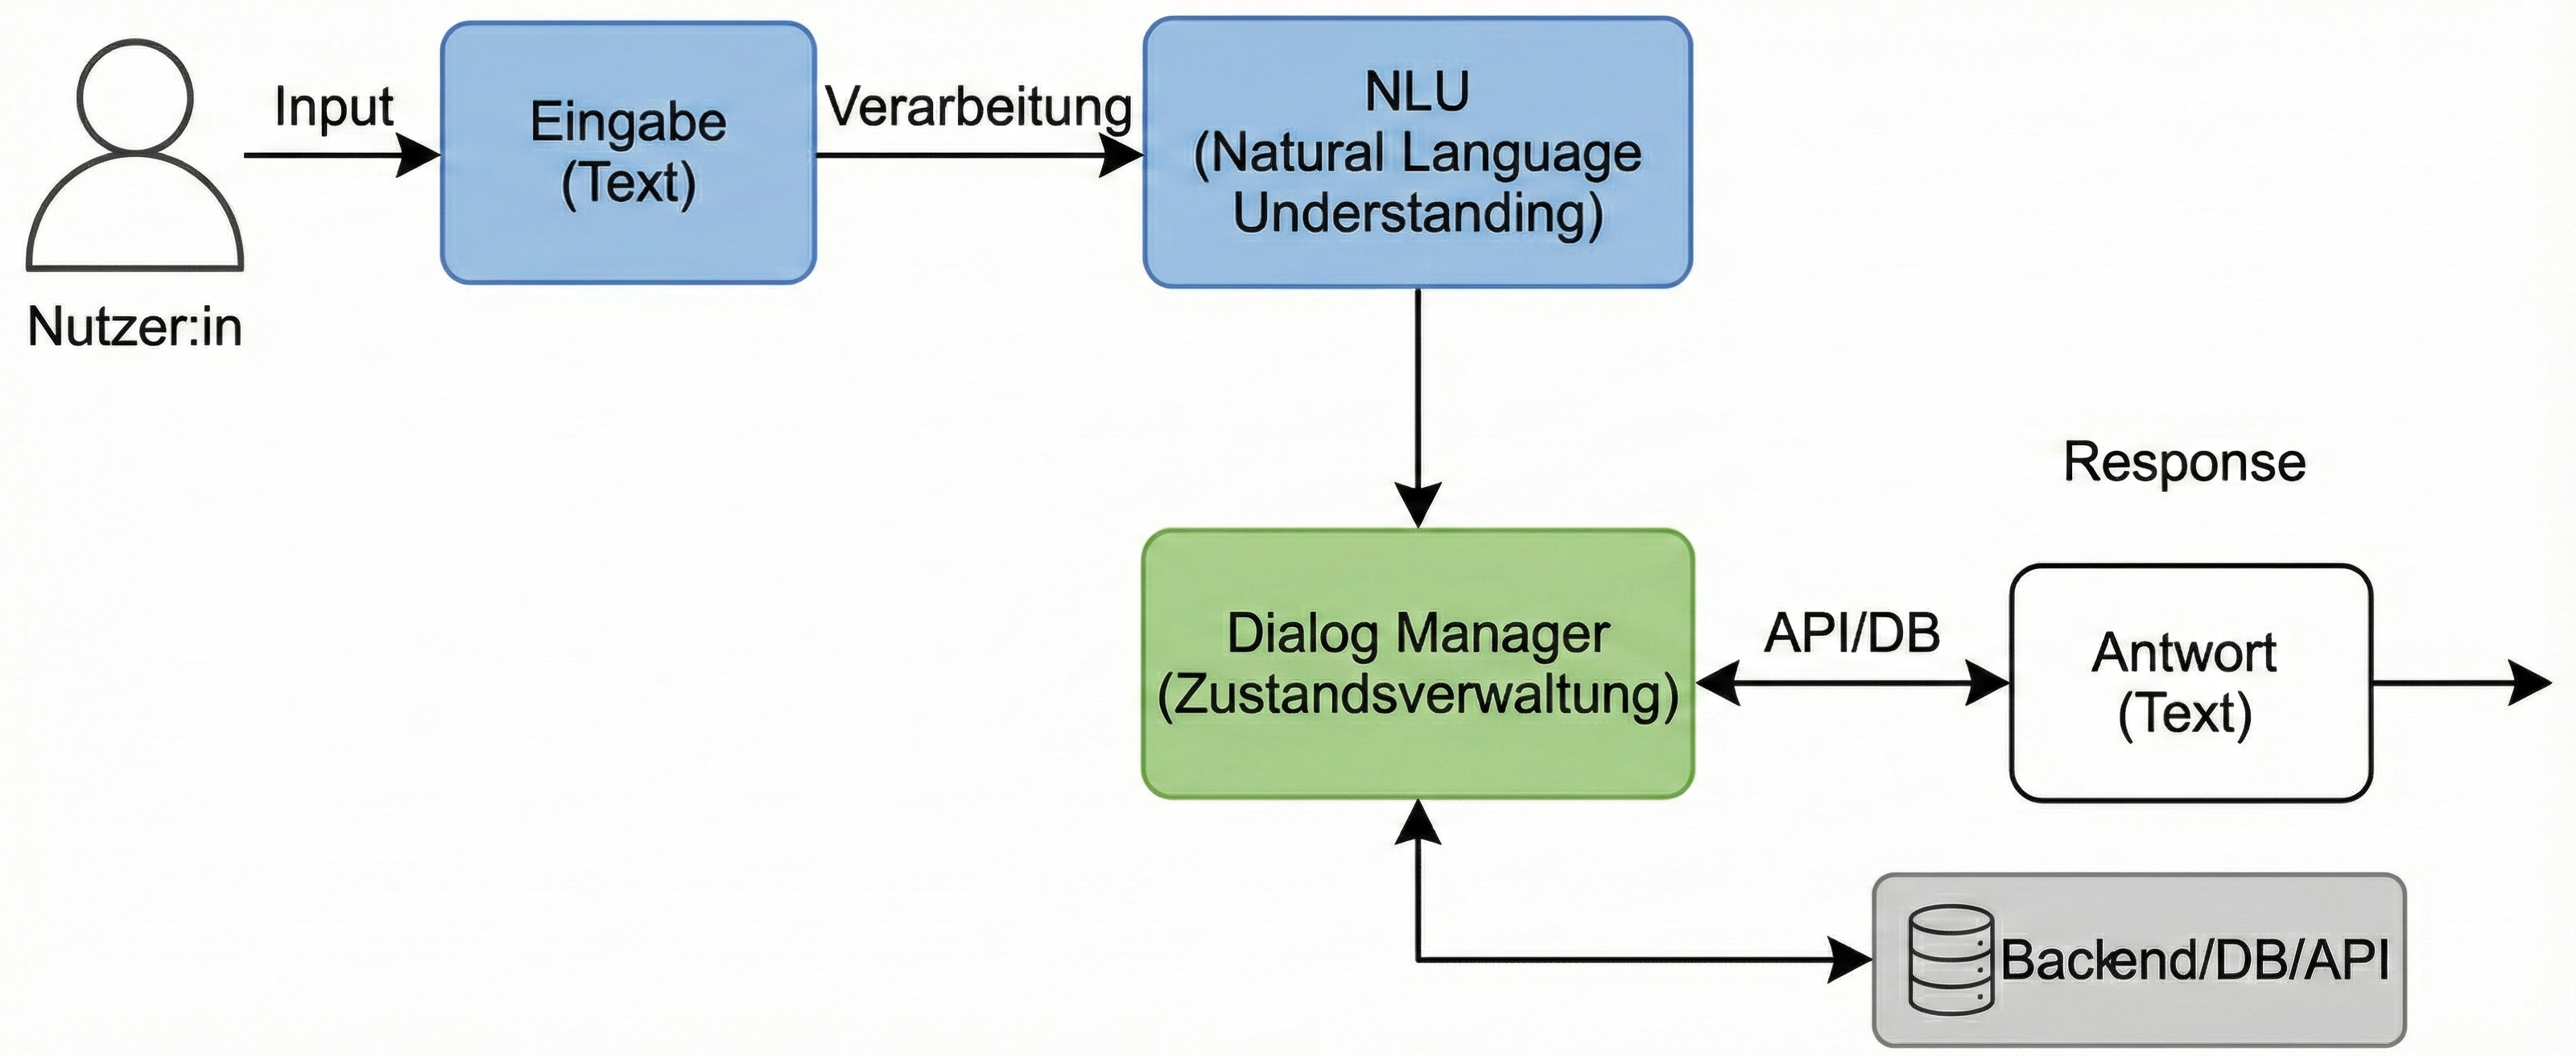
\includegraphics[width=0.92\textwidth]{chatbot_architektur.png}
\caption{Generische Architektur eines dialogbasierten Chatbots.}
\label{fig:chatbot_architektur}
\end{figure}

Zur konsistenten Führung von Dialogen wird häufig ein expliziter Dialogzustand verwaltet. Dieser wird beispielsweise in einer Sitzungsdatenbank gespeichert und ermöglicht es, Kontexte über mehrere Nachrichten hinweg aufrechtzuerhalten. In geschäftskritischen Szenarien werden Chatbots zusätzlich mit Validierungsmechanismen, klar definierten Dialogflüssen und Eskalationspfaden kombiniert. Auf diese Weise lassen sich sowohl eine hohe Nutzerfreundlichkeit als auch die erforderliche Prozesssicherheit gewährleisten.

Im Finanz- und Rechnungswesen werden Chatbots zunehmend zur Unterstützung wiederkehrender und stark strukturierter Aufgaben eingesetzt. Dazu zählen unter anderem die Beantwortung typischer Rückfragen, die Erfassung standardisierter Informationen oder das Anstoßen definierter Geschäftsprozesse. Ein wesentlicher Vorteil dialogbasierter Systeme besteht darin, dass sie über etablierte Kommunikationskanäle wie Messenger-Anwendungen verfügbar sind. Dadurch lassen sie sich ohne umfangreiche Schulungsmaßnahmen in bestehende Arbeitsabläufe integrieren. Die Interaktion verlagert sich hierbei von komplexen Formularoberflächen hin zu einer geführten, schrittweisen Datenerfassung im Dialog \cite{chatbots_finanzprozesse}.

Das in dieser Arbeit vorgestellte System nutzt diese Eigenschaften, indem ein Chatbot als zentrale, dialogbasierte Schnittstelle zur Erfassung von Rechnungs- und Dokumentendaten eingesetzt wird. Der Chatbot führt Nutzerinnen und Nutzer schrittweise durch den Erfassungsprozess, fragt fehlende Informationen gezielt ab und überprüft Eingaben unmittelbar auf Plausibilität. Die dabei gewonnenen strukturierten Daten werden anschließend an cloudbasierte Backend-Dienste übermittelt. Dort werden sie gespeichert, für die automatisierte Dokumentenerzeugung verwendet und in nachgelagerte Prozessschritte integriert. Auf diese Weise wird der Übergang von informeller Kommunikation, etwa einer kurzen Beschreibung der erbrachten Leistung per Text- oder Sprachnachricht, zu formalisierten Verwaltungsprozessen im Rechnungswesen weitgehend automatisiert und ohne Medienbrüche umgesetzt.

Daraus leitet sich für diese Arbeit die Anforderung ab, dass der Chatbot WhatsApp als etablierten Kanal nutzt, einen regelbasierten Dialogzustand mit Sitzungsdatenbank verwaltet und strukturierte Rechnungsdaten sicher extrahiert.




\section{Cloudbasierte Datenhaltung und Integrationen}
\label{sec:cloud-datenhaltung}
Cloudbasierte Datenhaltung bezeichnet die Speicherung von Informationen in extern betriebenen Rechenzentren, auf die über das Internet zugegriffen wird \cite{cloud_grundlagen}. Für kleine Dienstleistungsunternehmen und Einzelunternehmer entfällt dadurch der Bedarf an eigener Serverinfrastruktur, während Daten orts- und geräteunabhängig verfügbar sind. Wartung, Ausfallsicherheit und Skalierung werden weitgehend von spezialisierten Anbietern übernommen, sodass sich die Unternehmen stärker auf ihr Kerngeschäft konzentrieren können.

Ein zentrales Merkmal cloudbasierter Systeme sind standardisierte Programmierschnittstellen. Über solche Web-\glspl{ac:api} können unterschiedliche Anwendungen Daten lesen, schreiben und verarbeiten, ohne direkt auf die zugrunde liegende Infrastruktur zugreifen zu müssen. Web-Frontends, mobile Anwendungen und Automatisierungsdienste nutzen denselben Datenbestand, was Mehrfacherfassungen reduziert und konsistente Informationen in verschiedenen Nutzungskontexten ermöglicht.

Im Rechnungswesen kleiner Unternehmen erlaubt dieser Ansatz die Kombination spezialisierter Dienste statt eines monolithischen Systems. Eine cloudbasierte Datenbank kann etwa Kunden- und Rechnungsinformationen verwalten, während ein separater Speicherdienst für die Ablage von Dokumenten und eine Messaging-Plattform für die Kommunikation mit Nutzenden zuständig sind. Über Integrationslogik im Backend oder in Automatisierungsworkflows werden diese Komponenten zu einem durchgängigen Gesamtsystem verknüpft, in dem Daten zwischen den Diensten ausgetauscht und in unterschiedlichen Oberflächen wiederverwendet werden.

Für das in dieser Arbeit betrachtete Szenario bedeutet dies, dass Stammdaten, Rechnungsinformationen und Verweise auf Dokumente zentral in der Cloud geführt werden, während ergänzende Dienste wie Dokumentengenerierung und Dateispeicherung eigenständig, aber angebunden betrieben werden. Chatbot und Webanwendung greifen auf dieselben Daten zu und stoßen über integrierte Schnittstellen fachliche Prozesse an. Dadurch entsteht eine flexible Architektur, in der einzelne Dienste bei Bedarf ersetzt oder erweitert werden können, ohne die Gesamtstruktur grundlegend ändern zu müssen.





\section{Dokumentengenerierung in der Cloud}
\label{sec:dokumentengenerierung}
Unter Dokumentengenerierung in der Cloud wird die automatisierte Erstellung von Dateien wie Rechnungen, Angeboten oder Verträgen auf Basis digital vorliegender Daten verstanden. Anstatt Dokumente manuell in Textverarbeitungsprogrammen zu erstellen, werden strukturierte Informationen – etwa Kundenstammdaten, Positionslisten oder Zahlungsbedingungen – mit vordefinierten Vorlagen verknüpft. Die eigentliche Erzeugung des Dokuments erfolgt in einer Cloud-Umgebung, sodass keine lokale Bürosoftware erforderlich ist und die Erstellung jederzeit von verschiedenen Endgeräten ausgelöst werden kann.

Technisch basiert dieser Ansatz typischerweise auf Vorlagen, die Layout, Formatierung und feste Textbestandteile enthalten, während variable Inhalte über Platzhalter eingefügt werden.

Eine exemplarische Vorlage mit Platzhaltern ist in \autoref{fig:rechnung_vorlage} dargestellt.

\begin{figure}[H]
\centering
\includegraphics[width=0.85\textwidth]{rechnung_vorlage.png}
\caption{Google Docs Vorlage mit Platzhaltern für automatisierte Rechnungserstellung.}
\label{fig:rechnung_vorlage}
\end{figure}

 Bei der Generierung werden die Platzhalter durch konkrete Werte aus einem Datensystem ersetzt, wodurch aus einer einzigen Vorlage eine Vielzahl individueller Dokumente entstehen kann. Die Ausgabeformate reichen von bearbeitbaren Textdokumenten bis hin zu nicht veränderbaren Formaten wie \gls{ac:pdf}, die sich für den Versand an Kunden und für die revisionsorientierte Ablage eignen. Anpassungen am Erscheinungsbild oder an rechtlichen Pflichtangaben erfolgen zentral an der Vorlage und wirken sich unmittelbar auf alle zukünftigen Dokumente aus.

Die Cloud-Ausführung eröffnet zusätzliche Möglichkeiten der Integration in digitale Geschäftsprozesse. Dokumente können unmittelbar nach ihrer Erstellung automatisiert weiterverarbeitet werden, etwa durch Versand per E-Mail oder Messenger, Speicherung in strukturierten Ordnerhierarchien oder Übergabe an nachgelagerte Systeme wie Buchhaltung oder Dokumentenmanagement. Durch die enge Kopplung mit datenhaltenden Systemen und Workflows lassen sich manuelle Zwischenschritte deutlich reduzieren. Für kleine Unternehmen entsteht so ein durchgängiger Prozess von der Datenerfassung über die Dokumentenerzeugung bis zur Ablage, ohne dass Medienbrüche oder manuelle Formatierungsarbeit erforderlich sind \cite{dokumentengenerierung_cloud, google_docs_mailmerge}.

Für das entwickelte System wird daher eine Google Docs-Vorlage mit Platzhaltern verwendet, die automatisch mit Airtable-Daten befüllt und als PDF in Google Drive revisionssicher abgelegt wird.


\section{Grundlagen moderner Webanwendungen}
\label{sec:webanwendungen}
Moderne Webanwendungen unterscheiden sich deutlich von klassischen, statischen Websites. Während früher hauptsächlich einzelne HTML-Seiten ausgeliefert wurden, handeln aktuelle Anwendungen komplexe Geschäftslogik, dynamische Daten und interaktive Benutzeroberflächen im Browser. Grundlage ist dabei das Client–Server-Modell: Ein Webbrowser fungiert als Client, der über das \gls{ac:http}-Protokoll Anfragen an einen Server sendet. Der Server verarbeitet diese Anfragen, greift bei Bedarf auf Datenquellen zu und liefert strukturierte Antworten zurück, die im Frontend dargestellt oder weiterverarbeitet werden.

Auf der Client-Seite kommen typischerweise JavaScript-Frameworks zum Einsatz, die Single-Page-Applications (\gls{ac:spa}) ermöglichen. In einer \gls{ac:spa} wird die Benutzeroberfläche nicht bei jedem Seitenwechsel vollständig neu geladen, sondern dynamisch im Browser aktualisiert. Daten werden über asynchrone Anfragen an serverseitige Schnittstellen geladen und in Komponenten gerendert. Dieses Architekturprinzip erlaubt reaktionsschnelle Oberflächen, die sich in ihrer Bedienung eher wie klassische Desktop-Anwendungen verhalten und komplexe Interaktionen, etwa Tabellen mit Filter- und Sortierfunktionen, komfortabel abbilden \cite{webanwendungen_spa}.

Die serverseitige Ebene moderner Webanwendungen stellt meist klar definierte Programmierschnittstellen bereit, häufig in Form von \gls{ac:rest}- oder JSON-basierten \gls{ac:http}-\glspl{ac:api}. Darüber werden fachliche Operationen wie das Lesen, Anlegen oder Aktualisieren von Datensätzen kapsuliert. Ergänzend gewinnen serverlose Architekturen und sogenannte Edge Functions an Bedeutung, bei denen einzelne Funktionsbausteine ereignisgesteuert und skalierbar in einer Cloud-Umgebung ausgeführt werden. Sicherheitsmechanismen wie Authentifizierung und Autorisierung, Transportverschlüsselung sowie rollenbasierte Zugriffskonzepte sind integraler Bestandteil solcher Anwendungen und sorgen dafür, dass sensible Daten nur von berechtigten Nutzenden eingesehen oder verändert werden können.

Die ClientHub-Web-App nutzt dieses SPA-Prinzip mit React, TypeScript und Edge Functions für die strukturierte Darstellung von Kunden- und Rechnungsdaten aus Airtable sowie den Zugriff auf Drive-Dokumente.

% first example chapter
% @author Thomas Lehmann
%
\chapter{Technologischer Hintergrund}
\section{Make.com als Integrations- und Automatisierungsplattform}
\label{sec:make}

Make.com ist eine cloudbasierte Integrations- und Automatisierungsplattform,
die es ermöglicht, unterschiedliche Anwendungen, Dienste und Systeme
miteinander zu verbinden. Die Umsetzung erfolgt ohne klassische
Programmierung und basiert auf einem No-Code- beziehungsweise
Low-Code-Ansatz. Workflows werden in einer grafischen Benutzeroberfläche modelliert, indem vordefinierte Funktionsbausteine konfiguriert und zu logischen Abläufen
verknüpft werden. Dadurch können auch komplexe Integrationsprozesse ohne
umfangreiche Programmierkenntnisse umgesetzt werden.Aus technischer Sicht handelt es sich bei Make.com um eine Integrationsplattform, die externe Systeme über deren Web-APIs anbindet. Ereignisse und Datenflüsse werden dabei in einem zentralen
Orchestrierungslayer zusammengeführt und automatisiert verarbeitet.

Das zentrale Konstrukt in Make sind sogenannte Szenarien. Ein Szenario
beschreibt einen vollständigen Automatisierungsablauf, der aus einem
auslösenden Ereignis (Trigger), einer Abfolge von Verarbeitungsschritten
sowie einer oder mehreren Aktionen besteht.Die einzelnen Bausteine eines Szenarios werden als Module bezeichnet.
Diese repräsentieren entweder konkrete Anwendungsintegrationen, etwa zu
WhatsApp, Airtable oder Google Docs, oder generische Funktionen wie Filter,
Iteratoren, Aggregatoren oder Router. Trigger-Module starten ein Szenario
beispielsweise bei einer eingehenden Nachricht über einen Webhook. Aktionsmodule übernehmen anschließend die Verarbeitung der Daten, indem
sie Informationen lesen, schreiben oder an andere Systeme übertragen.
Mithilfe visueller Router und Filter können alternative Verarbeitungswege
modelliert werden, die abhängig von Dateninhalten oder Zuständen
unterschiedliche Pfade innerhalb des Szenarios durchlaufen.

Die Plattform stellt darüber hinaus erweiterte Funktionen zur
Ablaufsteuerung bereit. Mithilfe von Filtern können nur jene Datensätze
weiterverarbeitet werden, die definierte Bedingungen erfüllen, etwa das
Vorhandensein bestimmter Pflichtfelder. Iteratoren und Aggregatoren ermöglichen die Verarbeitung von Listenstrukturen. Dabei können Datensätze entweder einzeln durchlaufen
oder zu zusammengefassten Ergebnissen aggregiert werden. Router-Module
erlauben es, Workflows in mehrere Pfade zu verzweigen, die jeweils eigene
Bedingungen und nachgelagerte Verarbeitungsschritte besitzen. Auf diese Weise lassen sich auch komplexe und verzweigte Prozesse
modellieren, ohne dass eigener Kontrollfluss-Code implementiert werden
muss. Eine besondere Rolle nehmen Webhook-Trigger ein, da sie die nahezu
Echtzeit-Verarbeitung von Ereignissen aus externen Systemen ermöglichen,
sobald diese eine definierte URL aufrufen.

Im betrachteten Anwendungskontext fungiert Make.com als zentrale
Vermittlungsschicht zwischen Chatbot, Datenhaltung sowie Dokumenten- und
Speicherdiensten. Ereignisse aus der Kommunikationsschnittstelle werden
über Trigger-Module empfangen, innerhalb von Szenarien verarbeitet und
anschließend über Anwendungs-Module an Systeme wie Airtable, Google Docs
oder Google Drive weitergeleitet.Die Plattform übernimmt dabei die Steuerung der Datenflüsse, führt Validierungen aus und stößt nachgelagerte Aktionen an, etwa das Erzeugen
von Dokumenten oder das Aktualisieren von Datensätzen. Make.com erfüllt
damit die Rolle einer zentralen Orchestrierungsebene innerhalb der
Systemarchitektur. Insbesondere für kleinere Projekte und prototypische Anwendungen ergeben
sich daraus mehrere Vorteile. Die initiale Implementierung kann ohne
eigene Serverinfrastruktur erfolgen, vorgefertigte Konnektoren reduzieren
den Integrationsaufwand, und die Prozesslogik lässt sich durch die visuelle
Modellierung nachvollziehbar dokumentieren.

Gleichzeitig sind mit dem Einsatz einer Integrationsplattform wie Make.com
auch Einschränkungen verbunden. Sehr umfangreiche Szenarien können an
Übersichtlichkeit verlieren, da sämtliche Verarbeitungswege innerhalb
eines visuellen Diagramms abgebildet werden müssen. Zudem ist die
Abbildung komplexer Geschäftslogik nur eingeschränkt möglich. Darüber hinaus entsteht eine Abhängigkeit vom jeweiligen Anbieter, etwa
hinsichtlich Verfügbarkeit, Preisgestaltung und Funktionsumfang der
Plattform. Für hochskalierende oder besonders sicherheitskritische
Anwendungen kann daher eine klassisch implementierte, individuell
entwickelte Integrationsschicht sinnvoller sein. Make.com stellt hingegen insbesondere für klein- bis mittelkomplexe
Automatisierungsvorhaben mit begrenzten Ressourcen eine pragmatische und
gut nachvollziehbare Lösung dar.


\section{Airtable als Datenhaltung}
Airtable ist eine cloudbasierte Plattform, die tabellenorientierte
Benutzeroberflächen mit den Eigenschaften einer datenbankgestützten
Anwendung kombiniert. Aus Anwendersicht ähnelt Airtable einer klassischen
Tabellenkalkulation, erweitert diese jedoch um strukturierte Feldtypen,
Relationen zwischen Tabellen sowie eine standardisierte
Programmierschnittstelle. Dadurch eignet sich die Plattform insbesondere für Anwendungsszenarien, in denen Daten sowohl über eine webbasierte Oberfläche gepflegt als auch automatisiert von externen Systemen gelesen und geschrieben werden sollen.

Zentrale Konzepte in Airtable sind sogenannte Bases, die jeweils eine
in sich geschlossene Datenbankinstanz mit mehreren Tabellen
repräsentieren. Eine Tabelle besteht aus Datensätzen und Feldern, wobei
die Felder unterschiedliche Typen annehmen können, etwa Text, Zahl,
Datum, Auswahlfelder oder Verknüpfungen zu anderen Tabellen. Über verknüpfte Felder lassen sich einfache Relationen zwischen Tabellen modellieren, beispielsweise zwischen Kunden und zugehörigen Rechnungen. Darüber hinaus stehen verschiedene Sichten und Filter zur Verfügung, mit denen Teilmengen der Daten anhand frei definierbarer Kriterien angezeigt werden können. Formelfelder ermöglichen zudem die Berechnung dynamischer Werte. Sie können unter anderem zur Aggregation von Beträgen oder zur Erzeugung
formatierter Anzeigeinhalte eingesetzt werden.

Für den Einsatz als zentrale Datenhaltung in einem verteilten System ist
insbesondere die von Airtable bereitgestellte REST-API von Bedeutung. Sie
ermöglicht es, Datensätze programmatisch anzulegen, zu aktualisieren, zu
löschen oder anhand definierter Filterkriterien abzufragen. Auf diese Weise kann Airtable als zentrale „Single Source of Truth“ für fachliche Informationen fungieren. Unterschiedliche Frontends und Automatisierungsprozesse greifen dabei über die API auf denselben
konsistenten Datenbestand zu. Durch die Kombination aus grafischer Benutzeroberfläche und Programmierschnittstelle eignet sich Airtable sowohl für die manuelle
Pflege und Kontrolle von Daten als auch für die Integration in
automatisierte Workflows.

Im Kontext kleiner, cloudbasierter Anwendungen bietet Airtable mehrere
Vorteile gegenüber klassischen Datenbanksystemen. Die Tabellenstruktur
kann ohne aufwendige Deployment- oder Migrationsprozesse angepasst
werden, was insbesondere iteratives Arbeiten und prototypische
Entwicklungen erleichtert. Darüber hinaus unterstützt die grafische Benutzeroberfläche die manuelle Datenpflege sowie die Fehlersuche. Datensätze sind unmittelbar einsehbar
und bearbeitbar, wodurch einfache Auswertungen und Kontrollen direkt in
der Anwendung durchgeführt werden können. Demgegenüber stehen typische Einschränkungen gehosteter Plattformen. Dazu zählen unter anderem Begrenzungen hinsichtlich des maximalen Datenvolumens, der Anzahl zulässiger API-Aufrufe sowie die fehlende Unterstützung komplexer Transaktionen. Für klein- bis mittelkomplexe Anwendungen mit moderatem Datenumfang stellt Airtable dennoch eine pragmatische Lösung dar. Es ermöglicht die Realisierung einer zentralen, cloudbasierten Datenhaltung, ohne dass eine eigene Datenbankinfrastruktur betrieben werden muss.

\section{Google Docs und Google Drive}
Google Docs und Google Drive sind zentrale Bestandteile der
Google-Workspace-Plattform und bilden gemeinsam eine cloudbasierte
Umgebung zur Erstellung, Bearbeitung und Ablage von Dokumenten. Google
Docs stellt einen webbasierten Texteditor bereit, der die gleichzeitige
Bearbeitung eines Dokuments durch mehrere Personen ermöglicht.
Google Drive fungiert als zentraler Dateispeicher und bietet strukturierte
Ordner, Freigabefunktionen sowie Versionsverwaltung. Beide Dienste sind
vollständig browserbasiert und erlauben einen orts- und
geräteunabhängigen Zugriff auf Dokumente, ohne dass eine lokale
Office-Software installiert werden muss.




Für automatisierte Systeme ist insbesondere die Programmierschnittstelle
von Google Docs von Bedeutung. Sie ermöglicht es, Dokumente nicht nur
manuell, sondern auch programmatisch zu erzeugen und zu verändern. In der Praxis werden hierzu häufig Dokumentvorlagen verwendet, die das
Layout sowie feste Textbestandteile definieren. Variable Inhalte werden
über Platzhalter integriert, die bei der Dokumentenerstellung durch
konkrete Werte aus einem Datensystem ersetzt werden.
Auf diese Weise können aus einer einzelnen Vorlage eine Vielzahl
individueller Dokumente generiert werden. Typische Anwendungsfälle sind
unter anderem die standardisierte Erstellung von Rechnungen, Angeboten
oder Serienbriefen, ohne dass jedes Dokument manuell angepasst werden
muss.



Google Drive ergänzt diese Funktionalität durch eine strukturierte,
cloudbasierte Ablage der erzeugten Dokumente. Dateien können in
hierarchischen Ordnerstrukturen organisiert, mit Metadaten versehen und
über differenzierte Freigabemechanismen geteilt werden. Über die Google-Drive-API lassen sich Ordner und Dateien zudem programmgesteuert anlegen, verschieben, umbenennen dder herunterladen. Dadurch können Dokumentenerzeugung und Archivierung in einen
durchgängigen digitalen Prozess integriert werden. Insbesondere für kleinere Organisationen stellt Google Drive damit eine leichtgewichtige Alternative zu klassischen Dokumentenmanagementsystemen dar. Sowohl die manuelle Nutzung über die Weboberfläche als auch automatisierte Workflows auf Basis standardisierter Schnittstellen werden dabei unterstützt.




\section{Lovable Cloud / Supabase Edge Functions}
\section{Frontend-Stack (React, TypeScript, Tailwind, shadcn/ui)}
% first example chapter
% @author Thomas Lehmann
%
\chapter{Konzeption des Systems}
Dieses Kapitel beschreibt die Konzeption des zu entwickelnden Systems. Zunächst 
werden Anforderungen und zentrale Use Cases definiert. Anschließend wird die 
Zielarchitektur und Systemübersicht erläutert, gefolgt vom Datenmodell und 
den Datenflüssen. Darauf aufbauend folgt die detaillierte Beschreibung der 
Prozessabläufe „Rechnung neu erstellen" und „Dokument ablegen". Abschließend 
wird das Sicherheits- und Datenschutzkonzept vorgestellt.

\section{Anforderungen und Use Cases}
Die Situation und das Problem, das damit verbunden ist, sind wie folgt:

Das geplante System richtet sich vor allem an kleine Dienstleistungsfirmen, Einzelunternehmer sowie kleine und mittlere Gewerbebetriebe. Diese müssen regelmäßig Rechnungen erstellen und verwalten, verfügen jedoch weder über die Ressourcen noch über den Bedarf für umfassende Buchhaltungs- oder \glspl{ac:erp}-Systeme. Häufig mangelt es diesen Personen an IT-Kenntnissen und sie haben wenig Zeit. Deshalb benötigen sie einfache, zuverlässige und größtenteils automatisierte Prozesse. Auch Steuerberaterinnen und Steuerberater sind auf vollständig und strukturiert archivierte Rechnungsunterlagen angewiesen. Studien und Praxisanalysen zeigen, dass manuelle Rechnungsprozesse in kleinen Unternehmen mit einem erhöhten Zeitaufwand, einer höheren Fehleranfälligkeit sowie häufigen Medienbrüchen verbunden sind, was zu einem Mangel an Transparenz in den Abrechnungsprozessen führen kann \cite{bitkom_elektronische_rechnungsdaten_2022,beckit_rechnungsverarbeitung_2022,pleo_automatisierte_rechnungsverarbeitung_2024}.

In der Praxis erfolgt die Erstellung von Rechnungen und Dokumenten in vielen dieser Unternehmen überwiegend manuell. Die Ablage geschieht häufig in unsystematischen Ordnerstrukturen. Dieser Ansatz ist zeitaufwendig und anfällig für Fehler, da Kundendaten und Rechnungspositionen wiederholt neu eingegeben werden müssen. Dadurch steigt das Risiko von Zahlendrehern, unvollständigen Daten oder fehlerhaften Summenberechnungen. Zudem erschwert eine unstrukturierte Ablage das spätere Wiederfinden einzelner Dokumente, insbesondere wenn Belege zu einem späteren Zeitpunkt für buchhalterische oder steuerliche Zwecke benötigt werden.

Rechnungen, die Fehler aufweisen oder verspätet erstellt werden, können den Zahlungseingang verzögern und damit die Liquidität der Unternehmen beeinträchtigen. Sind Dokumente unvollständig, unsortiert oder schwer auffindbar, verlängert sich nicht nur die Bearbeitungszeit von Kundenanfragen – was den professionellen Außenauftritt beeinträchtigen kann –, sondern auch der Aufwand, wenn Belege kurzfristig benötigt werden. Die nachträgliche Aufbereitung und Abstimmung solcher Unterlagen kostet zusätzliche Zeit und Ressourcen und erhöht das Risiko, dass steuerliche Erklärungen fehlerhaft oder verspätet eingereicht werden.

Ziele und Anforderungen aus Sicht der Anwender

Die Entlastung im täglichen Verwaltungs- und Abrechnungsalltag steht aus Anwendersicht im Vordergrund.  Das Ziel ist es, die Zeit und den Aufwand, die für die Erstellung und Verwaltung von Rechnungen benötigt werden, deutlich zu reduzieren, damit mehr Zeit für das eigentliche Kerngeschäft bleibt.

 Gleichzeitig besteht das Bedürfnis nach einer übersichtlichen und verlässlichen Ablage für geschäftsrelevante Dokumente.  Um Fehler zu vermeiden und die Effizienz der Arbeitsabläufe zu verbessern, ist es entscheidend, dass alle Daten vollständig, korrekt und einheitlich erfasst werden.

 Außerdem ist die Zusammenarbeit mit externen Partnern, vor allem mit Steuerberaterinnen und Steuerberatern, von großer Bedeutung.  Anwender gehen davon aus, dass alle benötigten Unterlagen aktuell, vollständig und gut strukturiert sind, um Rückfragen zu minimieren und zusätzlichen Abstimmungsaufwand zu vermeiden. 

Diese Ziele resultieren in konkreten funktionalen Anforderungen an das System. Es muss den Nutzern ermöglichen, bestehende Kundendaten auszuwählen oder neue Kundendatensätze mit allen relevanten Stammdaten anzulegen. Darüber hinaus soll das System alle für die Rechnungserstellung erforderlichen Informationen erfassen. Dazu zählen unter anderem Leistungsbeschreibungen, Mengenangaben, Einzelpreise, Steuersätze und Zahlungsfristen, die strukturiert und nachvollziehbar eingegeben werden können.

Nach Abschluss der Datenerfassung stellt das System das erstellte Rechnungsdokument bereit und ermöglicht zudem die Ablage weiterer geschäftsrelevanter Dokumente, sodass diese später erneut abgerufen werden können.


Nicht nur die funktionalen, sondern auch die nicht-funktionalen Anforderungen sind von großer Bedeutung. Um auch Menschen ohne technische Vorkenntnisse zu erreichen, soll das System benutzerfreundlich gestaltet sein, sodass der Prozess der Rechnungserstellung und -verwaltung intuitiv durchlaufen werden kann. Eine positive Nutzungserfahrung setzt zudem kurze Reaktionszeiten voraus, um lange Wartezeiten für die Nutzer zu vermeiden.

Darüber hinaus ist es wichtig, dass das Erstellen neuer Rechnungen sowie das Ablegen von Dokumenten zügig erfolgt, damit erzeugte oder hochgeladene Dateien ohne spürbare Verzögerung zur Verfügung stehen. Das System muss außerdem zuverlässig und fehlertolerant arbeiten. Eingabefehler sollen durch geeignete Validierungen erkannt und abgefangen werden, während die Abläufe stabil und reproduzierbar ausgeführt werden.

Da personenbezogene Daten und Abrechnungsinformationen verarbeitet werden, kommt der Datensicherheit eine besondere Bedeutung zu. Zugangsdaten sind sicher zu speichern, die Kommunikation ist zu verschlüsseln und der Zugriff auf autorisierte Nutzer zu beschränken. Weiterhin soll die Systemarchitektur modular und erweiterbar gestaltet sein, um zukünftige Anforderungen oder zusätzliche Funktionen mit vertretbarem Aufwand integrieren zu können. Insgesamt orientiert sich das System damit an anerkannten Qualitätsmerkmalen nicht-funktionaler Anforderungen, wie sie im Qualitätsmodell der ISO/IEC 25010 sowie in der Fachliteratur beschrieben sind \cite{iso_25010_2023,seibert_nfa_2018,johann_nfa_2025}.


Anwendungsfall „Rechnung neu erstellen“

Der Anwendungsfall „Rechnung neu erstellen“ beginnt, sobald der Nutzer die entsprechende Aktion auswählt und den Erstellungsprozess startet. Zunächst entscheidet der Nutzer, ob die Daten eines bestehenden Kunden verwendet oder ein neuer Kundendatensatz angelegt werden soll. Bei der Neuanlage werden alle erforderlichen Stammdaten wie Name oder Firmenbezeichnung, Adresse, Kontaktinformationen und gegebenenfalls steuerliche Angaben erfasst.

Im nächsten Schritt gibt der Nutzer die zu fakturierenden Leistungen an. Dazu zählen die Leistungsbeschreibung sowie die zugehörigen Mengen, Einzelpreise und gegebenenfalls anwendbare Steuersätze. Der Nutzer kann mehrere Rechnungspositionen nacheinander erfassen, sofern dies erforderlich ist.

Anschließend werden rechnungsbezogene Angaben wie Rechnungsnummer, Rechnungsdatum, Leistungszeitraum und Zahlungsfrist festgelegt. Nach Abschluss der Dateneingabe wird die Rechnung erstellt und dem Nutzer zur Verfügung gestellt.



Anwendungsfall „Dokument ablegen“
Der Anwendungsfall „Dokument ablegen“ beginnt, sobald der Nutzer die entsprechende Aktion auswählt, um geschäftsrelevante Dokumente im System zu archivieren. Hierzu lädt der Nutzer eine Datei, beispielsweise einen Beleg oder eine Rechnung, hoch.

Das System ordnet das Dokument dem entsprechenden Kunden zu und legt es strukturiert ab, sodass es später zuverlässig wiedergefunden werden kann. Nach dem Abschluss des Vorgangs steht das abgelegte Dokument dem Nutzer zur Einsicht und zum erneuten Abruf zur Verfügung.
\begin{figure}[H]
\centering
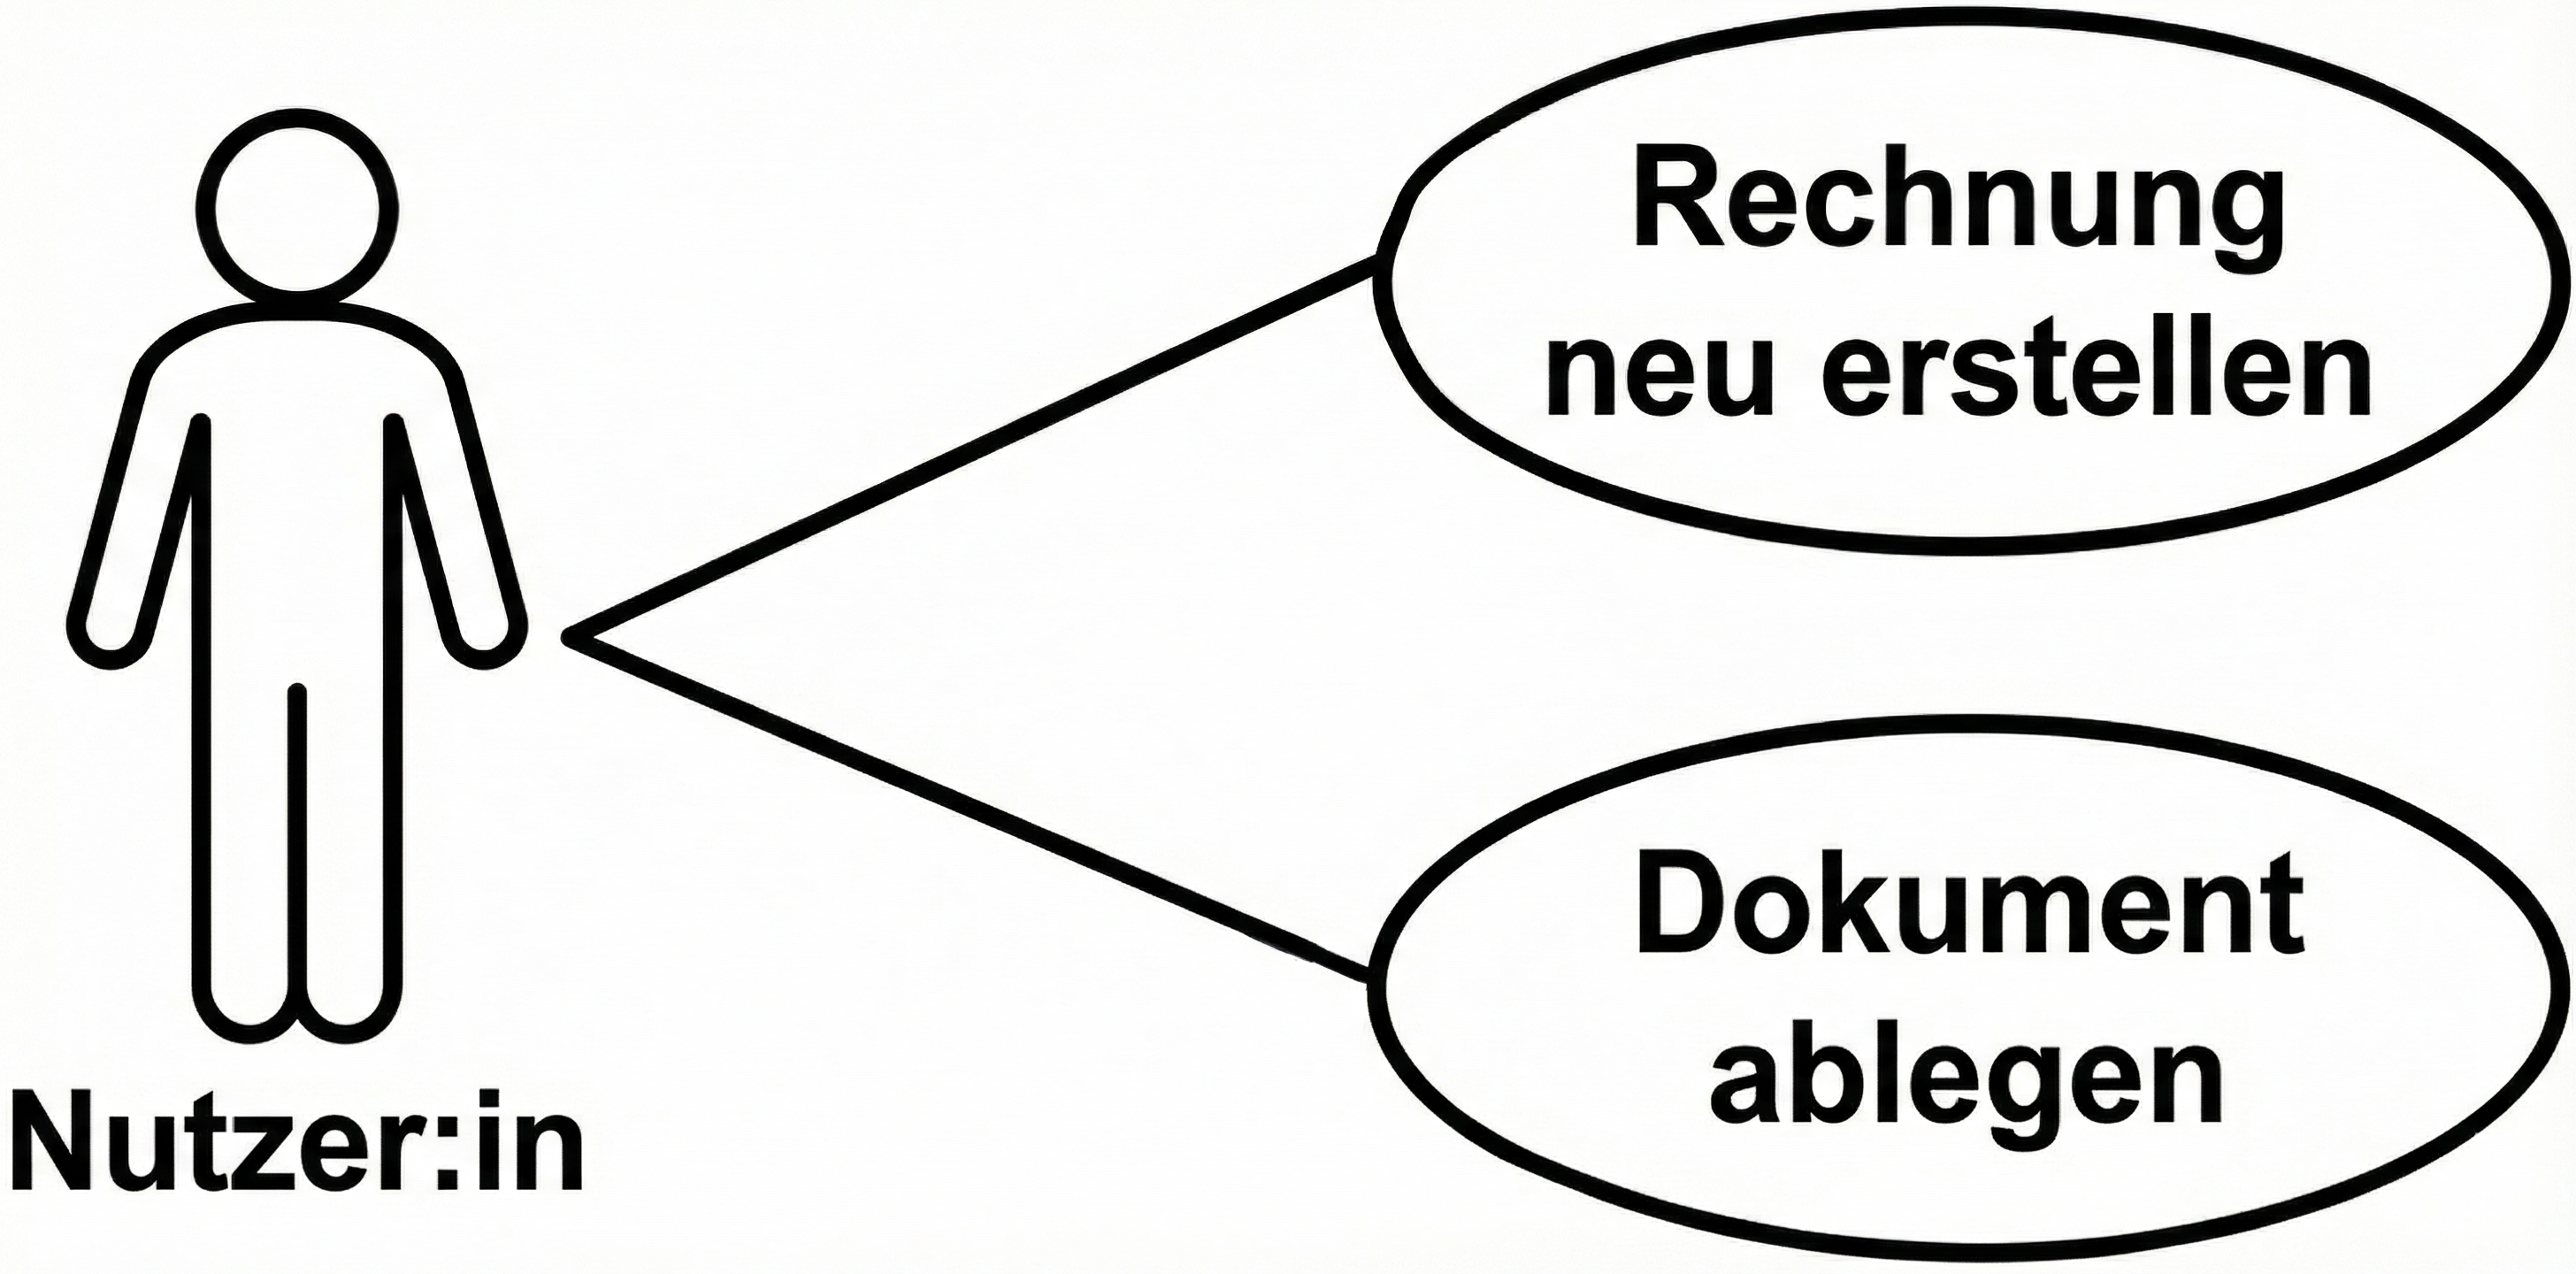
\includegraphics[width=0.8\textwidth]{use_case_diagramm.png}
\caption{Use Cases des Systems: Rechnungserstellung und Dokumentenablage.}
\label{fig:use_cases}
\end{figure}






\section{Zielarchitektur und Systemübersicht}
Die Zielarchitektur des Systems basiert auf mehreren klar abgegrenzten und lose gekoppelten Komponenten, die gemeinsam den End-to-End-Prozess der Rechnungs- und Dokumentenverarbeitung abbilden. Zu den zentralen Elementen zählen der WhatsApp-Chatbot zur Datenerfassung und Prozesssteuerung, Workflows auf der Automatisierungsplattform Make (make.com), eine Airtable-Datenbank als zentrale Datenquelle, Google Docs zur templatebasierten Dokumentenerstellung, Google Drive als Ablagesystem sowie die Web-Anwendung „ClientHub“ für Verwaltung und Zugriff.
Die einzelnen Komponenten sind überwiegend über standardisierte Cloud-\glspl{ac:api} miteinander verbunden. Dadurch können sie unabhängig voneinander betrieben und bei Bedarf flexibel erweitert werden.
\begin{figure}[H]
\centering
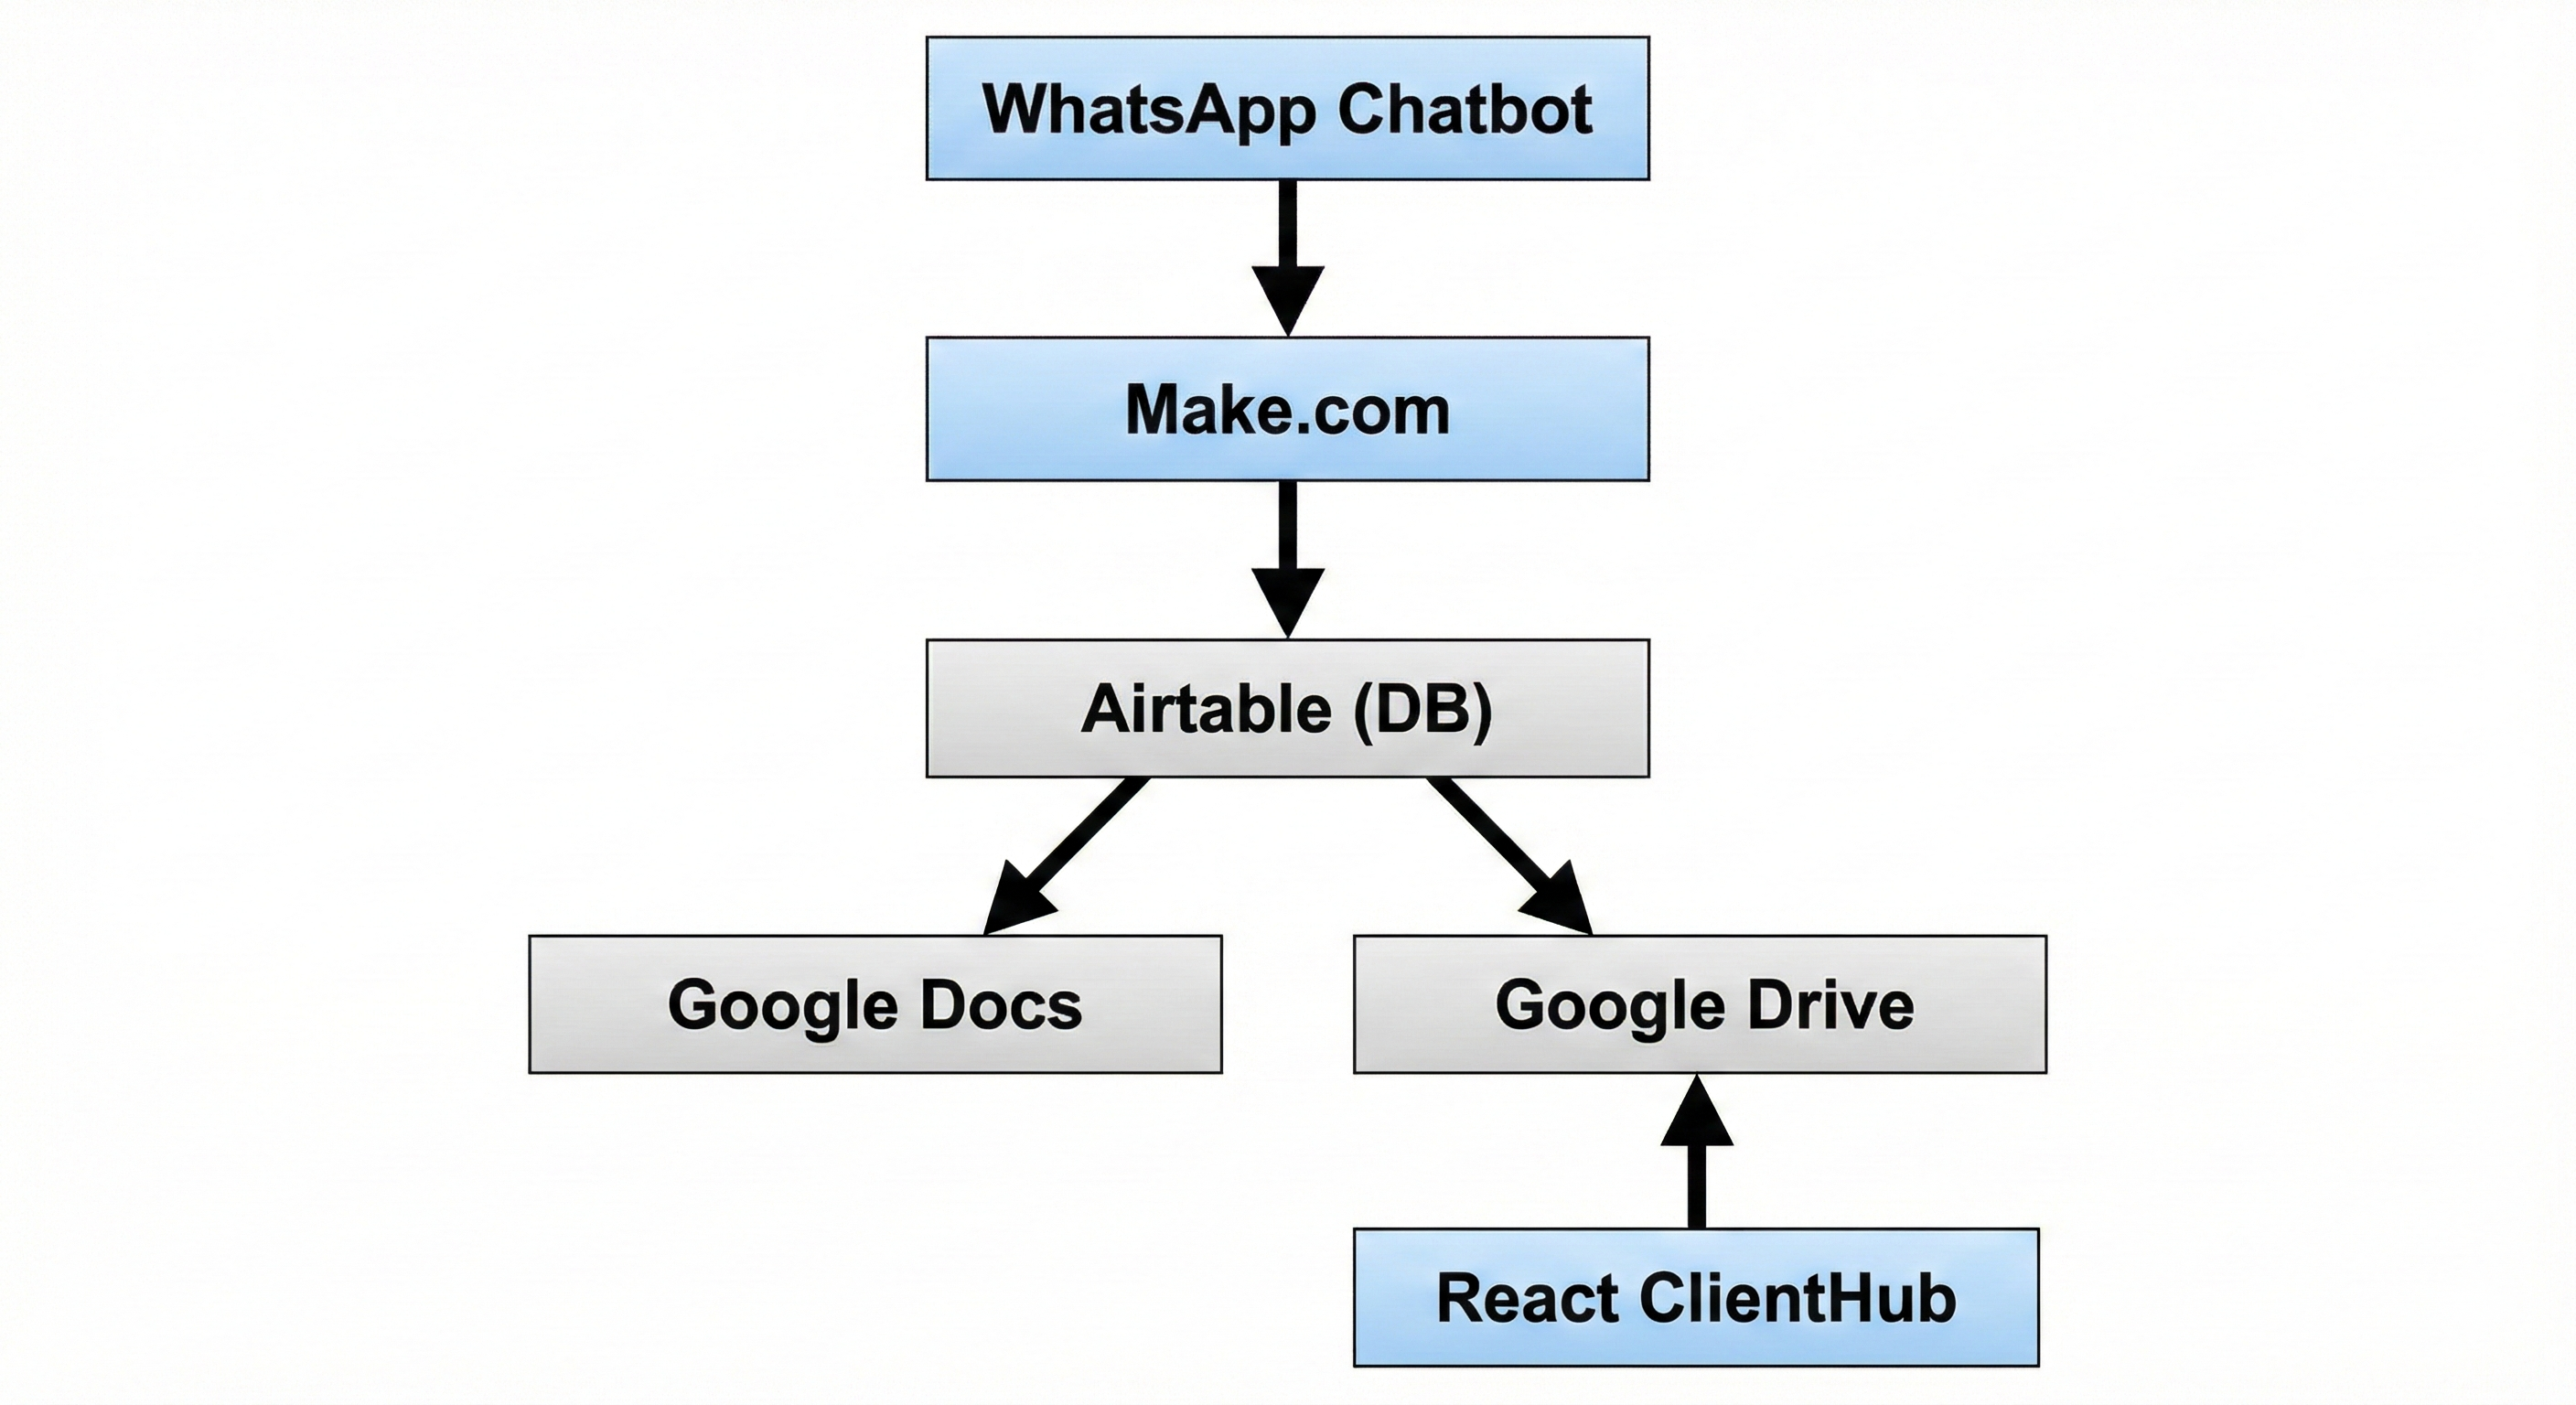
\includegraphics[width=0.9\textwidth]{systemarchitektur.png}
\caption{Zielarchitektur: WhatsApp Chatbot → Make.com → Airtable → Google Docs/Drive → React ClientHub.}
\label{fig:systemarchitektur}
\end{figure}

Das zentrale Element des Systems ist der Chatbot, der über WhatsApp erreichbar ist. Er begleitet die Nutzer dialoggesteuert durch den Prozess der Rechnungsgenerierung, indem er entsprechende Anweisungen gibt. Dies umfasst die Auswahl eines bestehenden Kunden oder die Erstellung eines neuen Kundendatensatzes, die Festlegung der Rechnungspositionen sowie die Bestimmung von Rechnungsnummer, Leistungszeitraum, Zahlungsfrist und Zahlungsart.
Ein weiteres Feature des Chatbots ist die Funktion „Dokument speichern“. Diese erlaubt es den Nutzern, Dateien wie Belege oder bereits erstellte Rechnungen hochzuladen, die anschließend im Kundenportal zur Verfügung gestellt werden. In beiden Szenarien leitet der Chatbot die erfassten Informationen in strukturierter Form an die nachgelagerten Arbeitsabläufe weiter. Er selbst führt keine direkten Abfragen an Datenbank- oder Speicherdiensten durch.

Eine Integrations- und Workflow-Plattform fungiert als Orchestrierungsschicht und implementiert die Logik der Automatisierung. Sie empfängt Nachrichten vom Chatbot, analysiert den aktuellen Dialogschritt und startet kontextabhängig unterschiedliche externe Dienste.
Hierzu zählen insbesondere die Airtable-\gls{ac:api} zur Erstellung und Aktualisierung von Kunden-, Rechnungs- und Sitzungsdaten (z. B. des aktuellen Prozessschritts) \cite{airtable_web_api_guide}, die Google-Docs-\gls{ac:api} zum Öffnen und Befüllen eines vordefinierten Rechnungsmusters sowie die Google-Drive-\gls{ac:api} zur Erstellung von Ordnern und zum Hochladen von Dateien. Ergänzend wird eine KI-Schnittstelle genutzt, um frei formulierte Texte oder Sprachnachrichten in strukturierte, deutschsprachige Rechnungspositionen zu überführen.
Im Rahmen des Dialogs weist der Nutzer die Rechnungsnummer zu. Diese wird als Feld in Airtable gespeichert, um sicherzustellen, dass sie in allen nachfolgenden Prozessschritten konsistent verwendet wird.

Google Drive fungiert als unabhängiges Speichersystem, das insbesondere im Anwendungsfall „Dokument ablegen“ genutzt wird. Der Nutzer startet diesen Vorgang, indem er über den Chatbot eine Datei hochlädt, die durch einen Workflow in eine kundenbezogene Ordnerstruktur überführt wird. Die Verzeichnisse sind nach Jahr, Quartal und Monat gegliedert; ist ein Ordner noch nicht vorhanden, wird er dynamisch erstellt.
Der archivierte Dateilink wird in Airtable gespeichert, sodass er für nachgelagerte Automatisierungen sowie für die Anzeige im Kundenportal verfügbar ist. Auf diese Weise entsteht eine konsistente und nachvollziehbare Archivierung, die sowohl interne Anforderungen als auch die Zusammenarbeit mit Steuerberaterinnen und Steuerberatern unterstützt.

Die Webanwendung „ClientHub“ ist eine browserbasierte React-Anwendung, die als eigenständiges Modul fungiert und ausschließlich serverseitige Edge-Funktionen nutzt, um auf externe Dienste zuzugreifen. Diese Edge-Funktionen bilden die Backend-Schicht der Architektur ab. Sie übernehmen die Interaktion mit der Airtable-\gls{ac:api} und der Google-Drive-\gls{ac:api}, bereiten die Daten für das Frontend auf und schützen gleichzeitig sensible Zugangsdaten vor einem direkten Zugriff aus dem Browser.
Die Webanwendung stellt den Nutzern ein Dashboard mit aggregierten Metriken zur Verfügung. Darüber hinaus bietet sie eine Kundenliste mit Such- und Filteroptionen sowie eine Übersicht über die Ordnerstruktur des Kundenportals, über die archivierte Dokumente eingesehen und heruntergeladen werden können.

Das Design folgt bewusst den architektonischen Grundsätzen der losen Kopplung, der Modularität und der klaren Schichtentrennung. Die Frontend-Logik, die Orchestrierung der Integrationsprozesse und die Datenhaltung sind voneinander entkoppelt. Dadurch können Änderungen in einer Komponente, wie etwa der Austausch des Chatkanals oder die Erweiterung der Datenstruktur, mit nur minimalen Anpassungen in den übrigen Systemteilen umgesetzt werden.
Durch den konsequenten Einsatz von Cloud-Diensten und standardisierten \glspl{ac:api} ist keine eigene Serverinfrastruktur erforderlich. Betrieb, Skalierung und Verfügbarkeit werden größtenteils von den jeweiligen Plattformanbietern übernommen. Die Architektur weist damit Eigenschaften auf, die sie besonders geeignet für kleine Unternehmen machen, die mit begrenzten Ressourcen arbeiten, einen geringen Wartungsaufwand benötigen und dennoch eine Lösung suchen, die flexibel mit wachsenden Anforderungen erweitert werden kann. Lose Kopplung, Modularität und eine klare Schichtentrennung gelten in der Softwarearchitektur als wesentliche Voraussetzungen für wartbare und erweiterbare Systeme. \cite{balzert_softwaretechnik_2011}.
Der konsequente Einsatz wohldefinierter \glspl{ac:api} wird als zentraler Baustein integrationsfähiger, verteilter Systeme beschrieben \cite{spichale_apidesign_2020}.


\section{Datenmodell und Datenflüsse}

Das zugrunde liegende Datenmodell und die zentralen Datenflüsse, die die dialogbasierte Rechnungserstellung sowie die Ablage geschäftsrelevanter Dokumente unterstützen, werden im folgenden Abschnitt erläutert. Die Daten werden in mehreren Airtable-Tabellen gespeichert, die gemeinsam den Chatbot-Dialog, die Rechnungserstellung und die Dokumentenablage in Google Drive abbilden. Die Tabellen dienen dabei nicht nur als persistenter Speicher fachlicher Informationen, sondern bilden zugleich die Grundlage für die Steuerung der Workflows in der Automatisierungsplattform, indem sie Zustandsinformationen und temporäre Eingaben strukturiert bereitstellen.

Im Datenmodell steht die Tabelle „User\_Sessions“ im Mittelpunkt. Sie fungiert als zentrale Instanz zur Verwaltung von Nutzerzuständen und zur Zugriffskontrolle innerhalb des Chatbot-Workflows. In dieser Tabelle werden die Telefonnummern der Nutzer gespeichert, sodass eingehende WhatsApp-Nachrichten validiert und ausschließlich registrierte Rufnummern zum Systemzugang zugelassen werden. Darüber hinaus enthält „User\_Sessions“ Zustandsvariablen wie „Current Step“ und „Next Step“, die zur Steuerung des dialogbasierten Ablaufs verwendet werden. Diese Informationen sind erforderlich, da die eingesetzte Automatisierungsplattform lediglich ein einzelnes Watch-Event für eingehende Nachrichten bereitstellt und keine native Unterstützung für eine zustandsabhängige Dialogführung bietet.
\begin{figure}[H]
\centering
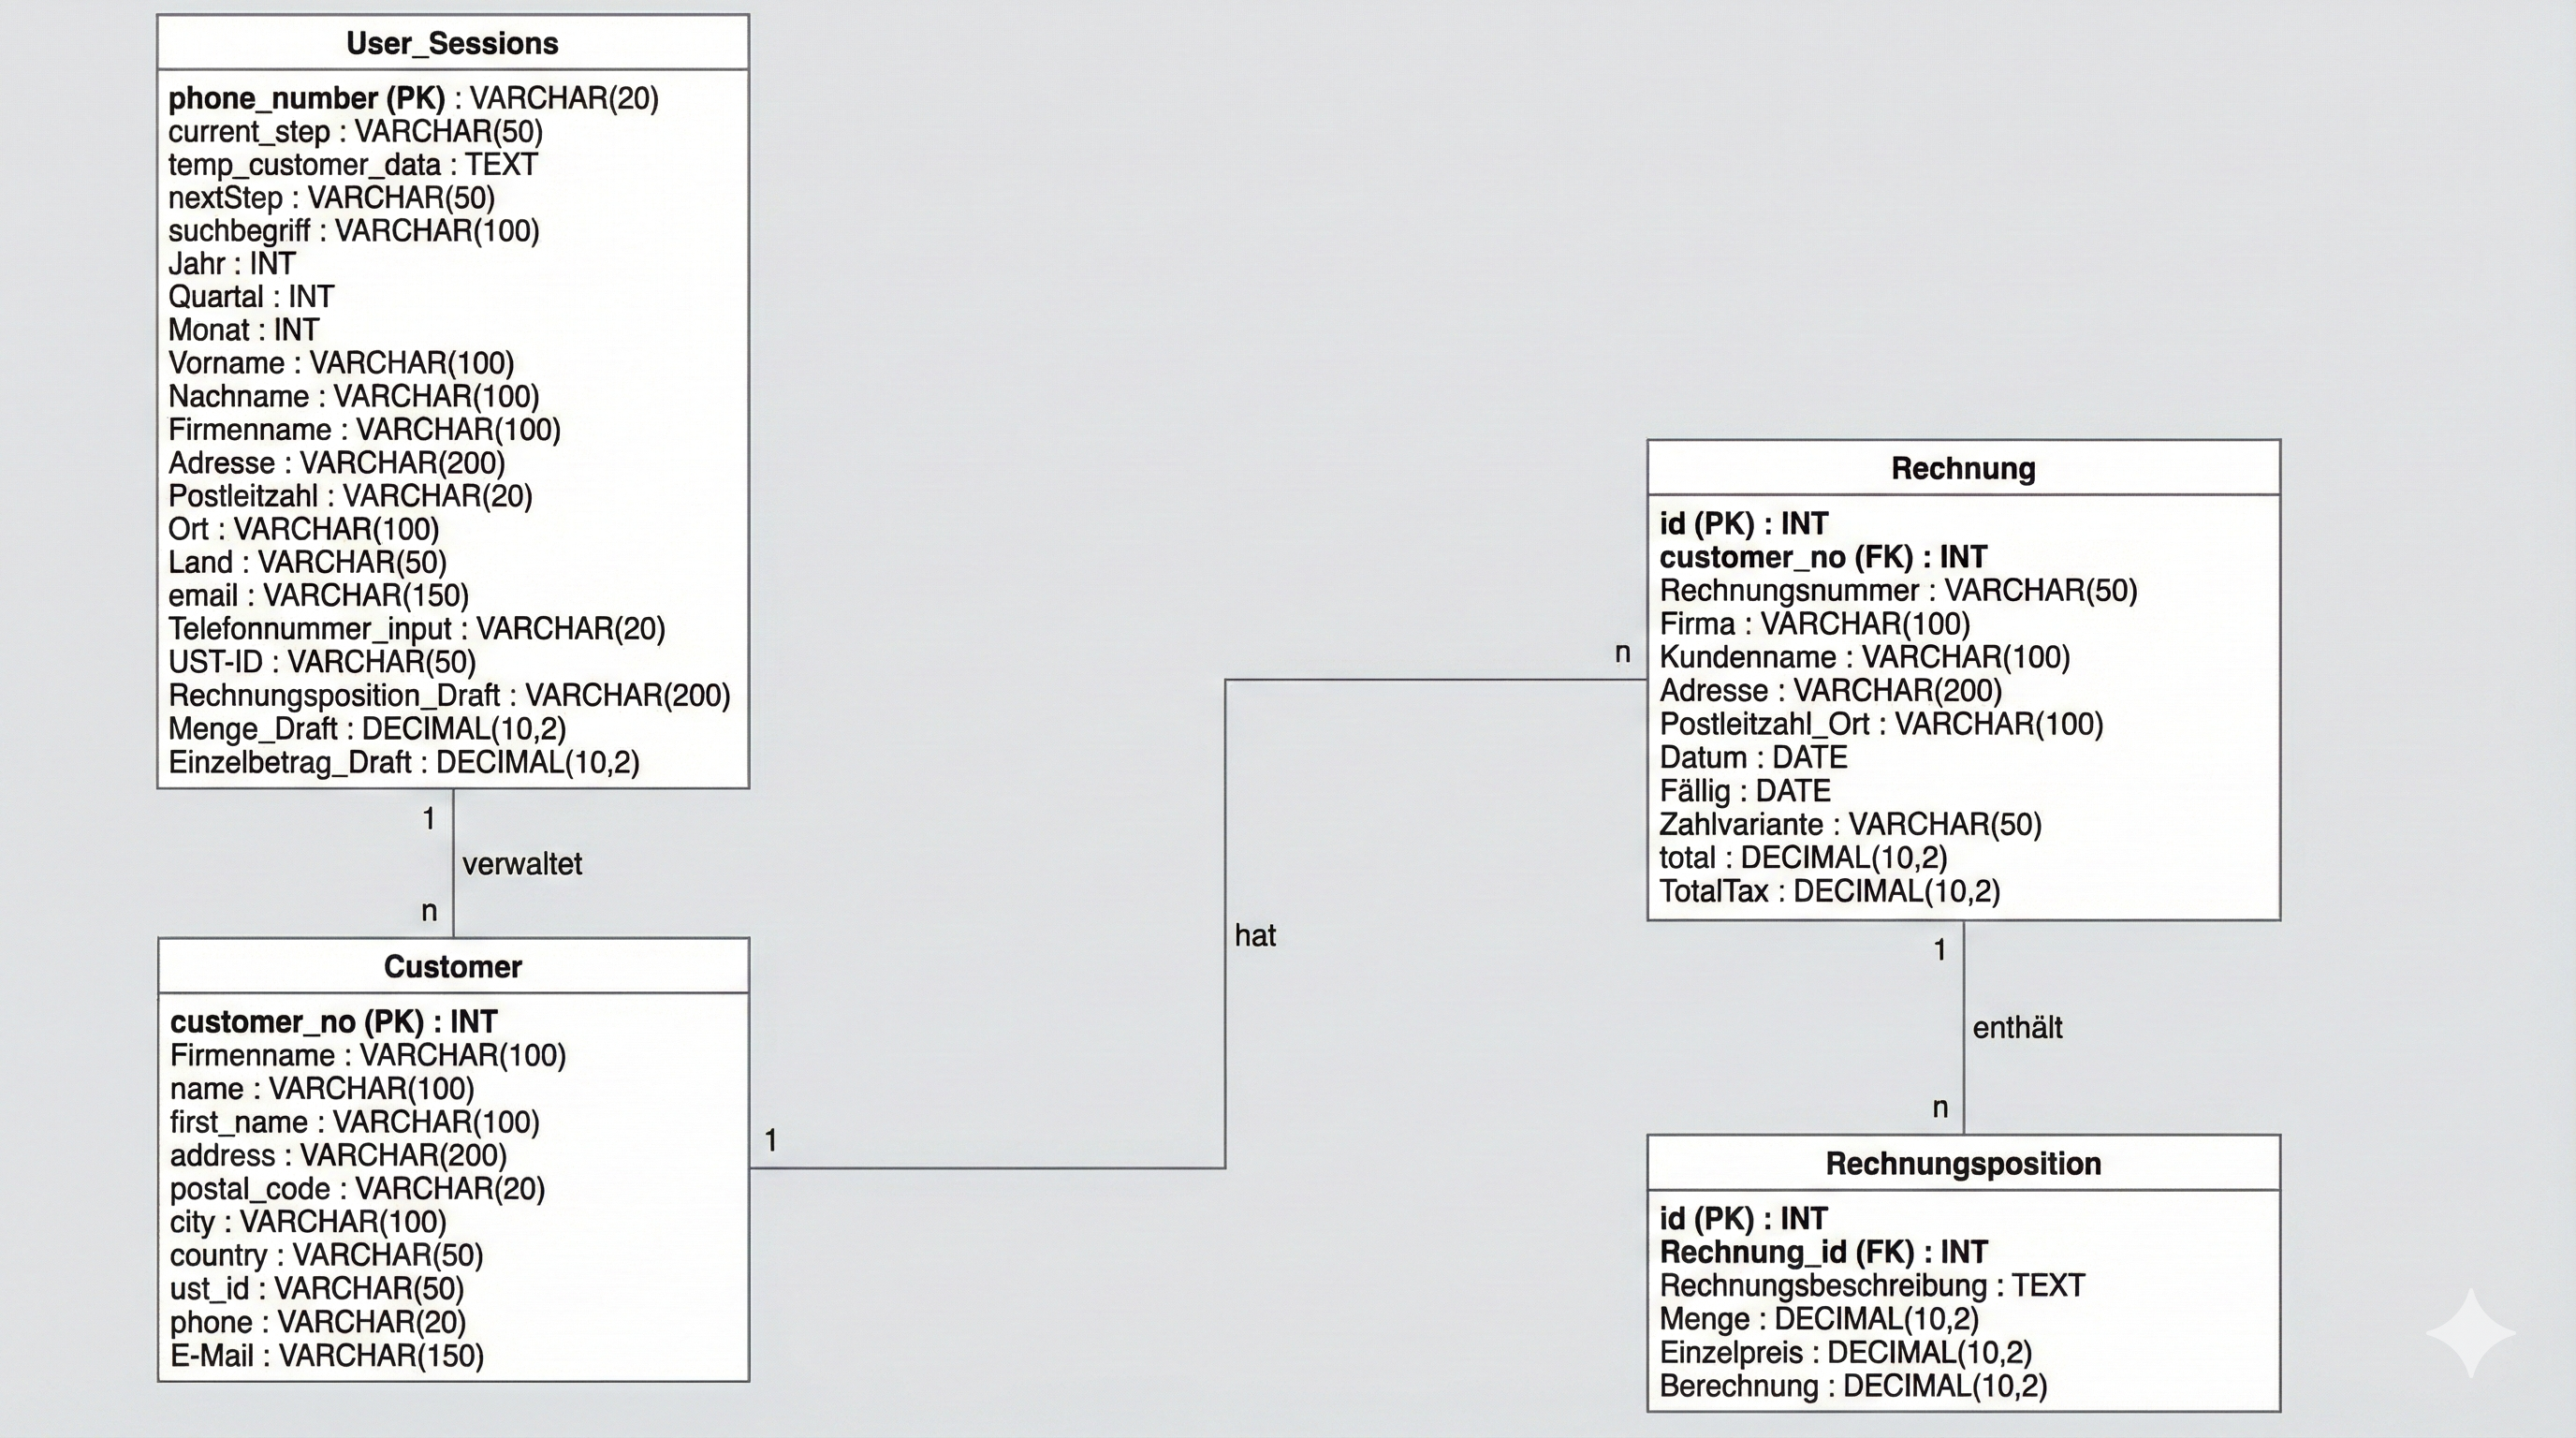
\includegraphics[width=0.9\textwidth]{datenmodell_er.png}
\caption{Airtable-Datenmodell mit Relationen (User\_Sessions, Customer, Rechnung, Rechnungsposition).}
\label{fig:datenmodell}
\end{figure}


„User\_Sessions“ enthält ausschließlich dynamische, während des Gesprächsverlaufs veränderliche Felder. Diese dienen der temporären Speicherung von Nutzereingaben und ermöglichen eine iterative, dialogorientierte Datenerfassung. Ein zentrales Ziel dieser Struktur besteht darin, Korrekturen und Anpassungen durch die Nutzenden jederzeit zuzulassen. Gibt eine Person beispielsweise versehentlich ein falsches Rechnungsjahr an, kann dieser Wert direkt im Chat korrigiert werden. Der entsprechende Eintrag in „User\_Sessions“ wird aktualisiert, und der Workflow setzt mit den korrigierten Daten fort, ohne dass der gesamte Dialog erneut durchlaufen werden muss.

Ein vergleichbares Vorgehen wird bei der Neuanlage von Kunden angewendet. Temporäre Felder wie Vorname, Nachname, Adresse, Postleitzahl und Umsatzsteuer-Identifikationsnummer werden zunächst schrittweise erfasst und können bei Bedarf angepasst werden. Erst nachdem alle erforderlichen Felder vollständig ausgefüllt und eine automatisch generierte Zusammenfassung der Kundendaten explizit bestätigt wurde, erfolgt die dauerhafte Speicherung des Kunden in einer separaten Kundentabelle. Auch rechnungsbezogene Parameter wie Leistungsbeschreibung, Menge und Einzelpreis werden zunächst in „User\_Sessions“ zwischengespeichert. „User\_Sessions“ fungiert somit als transiente Datenspeicherschicht, die keine dauerhafte Persistenz besitzt, sondern ausschließlich der Dialogsteuerung und der Vorbereitung der eigentlichen Geschäftsobjekte dient.

Die dauerhaft gültigen Kundendaten werden in der Tabelle „Customer“ verwaltet, die als zentrale Kundendatenbank des Systems dient. Neue Kundendatensätze können sowohl über die Webanwendung als auch direkt über den Chatbot angelegt werden. In dieser Tabelle werden alle für die Rechnungsstellung relevanten Stammdaten gespeichert, darunter Vor- und Nachname, Firmenbezeichnung, vollständige Adresse, E-Mail-Adresse, Telefonnummer sowie die Umsatzsteuer-Identifikationsnummer. Nach Abschluss eines Neuanlage-Dialogs werden die zuvor in „User\_Sessions“ erfassten temporären Kundendaten in einen konsistenten Datensatz in „Customer“ überführt. Bestehende Kunden werden über ihre in der Tabelle hinterlegten Attribute identifiziert und können im Dialog ausgewählt werden, sodass die bereits gespeicherten Stammdaten ohne erneute Eingabe für die Rechnungserstellung genutzt werden.

Die eigentliche Rechnungslogik ist in den Tabellen „Rechnung“ und „Rechnungsposition“ abgebildet. Die Tabelle „Rechnung“ speichert alle kopfbezogenen Informationen einer Rechnung, insbesondere den zugehörigen Kunden, die Rechnungsnummer, das Rechnungsdatum, den Leistungszeitraum, die Fälligkeit der Forderung sowie die gewählte Zahlungsart. Die hierfür erforderlichen Daten stammen einerseits aus der Tabelle „Customer“, andererseits aus den während des Dialogs in „User\_Sessions“ gespeicherten Eingaben und ergänzenden Feldern, die direkt im Chat erfasst und an Airtable übergeben werden. Zusätzlich werden in „Rechnung“ aggregierte Beträge gespeichert, indem die Summe aller zugehörigen Rechnungspositionen aus der Tabelle „Rechnungsposition“ übernommen und als Grundlage für die Berechnung des Bruttobetrags einschließlich Umsatzsteuer verwendet wird. Diese Berechnungen erfolgen über Formel-Felder, die den Nettobetrag mit einem vordefinierten Steuersatz multiplizieren und auf zwei Nachkommastellen runden.

Die Tabelle „Rechnungsposition“ erfasst die einzelnen Positionen einer Rechnung. Für jede Position werden Daten wie die Leistungsbeschreibung, die Menge und der Einzelpreis gespeichert, die zuvor dialogbasiert erhoben und in „User\_Sessions“ zwischengespeichert wurden. Die Berechnung des Positionsbetrags erfolgt über ein Formel-Feld, indem die Menge mit dem numerischen Einzelpreis multipliziert wird. Da eine Rechnung typischerweise mehrere Positionen umfassen kann, werden für jede Position separate Datensätze angelegt. Die Zuordnung der einzelnen Rechnungspositionen zu einer Rechnung erfolgt über Referenzinformationen wie die Rechnungsnummer oder interne Identifikatoren innerhalb der Workflow-Logik, ohne dass zwingend explizite Verknüpfungsfelder im Airtable-Schema definiert werden müssen.

Der Datenfluss im Anwendungsfall „Rechnung neu erstellen“ beginnt mit dem Eingang einer WhatsApp-Nachricht, mit der der Nutzer den Erstellungsprozess startet. Zunächst wird eine neue Sitzung in „User\_Sessions“ angelegt oder eine bestehende Sitzung aktualisiert, indem die Telefonnummer gespeichert und die Zustandsvariablen initialisiert werden. Anschließend werden alle für die Rechnungserstellung erforderlichen Informationen dialogbasiert erhoben und in den dynamischen Feldern von „User\_Sessions“ zwischengespeichert, darunter Kundendaten, Leistungsbeschreibungen, Mengen, Einzelpreise, Rechnungsdatum, Leistungszeitraum und Zahlungsfrist. Sobald alle Kundendaten vollständig vorliegen und bestätigt wurden, überführt der Workflow die temporären Angaben in einen dauerhaften Datensatz in „Customer“, sofern ein neuer Kunde anzulegen ist. Bei bestehenden Kunden wird lediglich der entsprechende Datensatz referenziert.

Im nächsten Schritt erzeugt der Workflow einen neuen Eintrag in der Tabelle „Rechnung“ und legt parallel für jede erfasste Rechnungsposition einen Datensatz in „Rechnungsposition“ an, der die zuvor zwischengespeicherten Leistungsdaten übernimmt. Nach Abschluss der Positionserfassung werden in „Rechnung“ die relevanten Summen berechnet, indem die Beträge der zugeordneten Positionen aggregiert und um die Umsatzsteuer ergänzt werden. Auf Basis dieser Daten wird in Google Docs ein Rechnungsdokument auf Grundlage eines vordefinierten Templates generiert, das die aus Airtable stammenden Felder einfügt und anschließend über die Google-Drive-\gls{ac:api} als \gls{ac:pdf} exportiert wird \cite{google_docs_api,google_drive_files_export_2025}.
 Das fertige Dokument wird dem Nutzer über den Chat zur Verfügung gestellt und kann für weitere Prozesse, etwa die Ablage oder den Versand, verwendet werden.

Der Datenfluss im Anwendungsfall „Dokument ablegen“ ist ebenfalls dialoggesteuert, fokussiert sich jedoch auf die strukturierte Archivierung von Dateien. Der Prozess wird durch das Hochladen eines Dokuments, beispielsweise eines Belegs oder einer externen Rechnung, über den WhatsApp-Chatbot initiiert. Im Dialog werden die zur Zuordnung notwendigen Informationen erfasst, insbesondere der betroffene Kunde sowie der zeitliche Kontext der Ablage (Jahr, Quartal, Monat), und temporär in einer Sitzung gehalten. Auf Basis dieser Parameter erstellt der Workflow die entsprechende Ordnerstruktur in Google Drive, sofern diese noch nicht existiert, und lädt das Dokument in den kundenbezogenen Unterordner hoch.

Der dabei erzeugte Dateilink steht dem System für nachgelagerte Schritte zur Verfügung, etwa zur Anzeige im Kundenportal. Durch diesen Ablauf wird sichergestellt, dass hochgeladene Dokumente konsistent, nachvollziehbar und eindeutig in Bezug auf Kunde und Zeitraum zugeordnet werden können, ohne dass manuell eine eigene Ablagestruktur gepflegt werden muss.

\section{Prozessablauf vom Chatbot bis zur Ablage}
\subsection{Ablauf „Rechnung neu erstellen“}
In diesem Unterabschnitt wird der Ablauf des Anwendungsfalls „Rechnung neu erstellen“ beschrieben. Der Prozess beginnt mit der Interaktion der Nutzerinnen und Nutzer im WhatsApp-Chat. Anschließend werden die erforderlichen Rechnungsdaten schrittweise erfasst und gespeichert. Auf dieser Grundlage wird ein Rechnungsdokument erstellt, das den Nutzern am Ende des Prozesses als \gls{ac:pdf} direkt im Chat zur Verfügung gestellt wird.

Der Ablauf beginnt, sobald der Nutzer nach der initialen Verifizierung im WhatsApp-Chat den Befehl \glqq Start\grqq{} sendet und im angezeigten Hauptmenü die Option \glqq Rechnung erstellen\grqq{} auswählt. Anschließend wird in der Tabelle \texttt{User\_Sessions} ein Sitzungseintrag angelegt oder aktualisiert. Das Zustandsfeld \texttt{current\_step} wird dabei auf den entsprechenden Wert gesetzt, um den weiteren Dialogverlauf zu steuern.
Auf Basis dieses Sitzungszustands führt der Chatbot den Nutzer schrittweise durch den Prozess. Nach jeder Eingabe wird gezielt die nächste passende Frage gestellt und der aktuelle Zustand entsprechend aktualisiert.


Im ersten inhaltlichen Schritt entscheidet der Nutzer, ob ein neuer Kunde angelegt oder ein bestehender Kunde ausgewählt werden soll. Wird die Option zur Neuanlage gewählt, führt der Chatbot den Nutzer schrittweise durch die Erfassung der erforderlichen Stammdaten.
Dabei wird jedes Datenfeld einzeln abgefragt und zunächst temporär in der Tabelle \texttt{User\_Sessions} gespeichert. Am Beispiel des Vornamens wird dieser Wert nach der Eingabe in einem dynamischen Feld hinterlegt und anschließend durch eine Bestätigungsfrage (\glqq Ist der eingegebene Vorname korrekt?\grqq{}) verifiziert. Abhängig von der Antwort wird entweder der nächste Dialogschritt eingeleitet oder die Eingabe erneut abgefragt.
Dieses Vorgehen wird analog für weitere Stammdaten wie Nachname, Firmenname, Adresse, Postleitzahl, Ort, Land, E\hyp{}Mail\hyp{}Adresse, Telefonnummer sowie die Umsatzsteuer\hyp{}Identifikationsnummer angewendet. Nachdem alle erforderlichen Angaben vollständig erfasst und bestätigt wurden, werden die gesammelten Daten aus \texttt{User\_Sessions} in einen neuen, dauerhaften Datensatz in der Tabelle \texttt{Customer} überführt. Gleichzeitig werden die kopfbezogenen Kundendaten für die spätere Erstellung der Rechnungsvorlage vorbereitet.


Entscheidet sich der Nutzer für die Auswahl eines bestehenden Kunden, wird zunächst ein Suchbegriff abgefragt und in der Tabelle \texttt{User\_Sessions} gespeichert. Auf Grundlage dieses Suchbegriffs werden passende Kundendatensätze ermittelt, woraufhin der Chatbot unterschiedliche Dialogpfade anbietet.
Ergibt die Suche keinen Treffer, kann der Nutzer entweder einen neuen Kunden anlegen, einen weiteren Suchversuch starten oder den Vorgang abbrechen. Führt die Suche zu genau einem Ergebnis, kann dieser Kundendatensatz direkt übernommen oder eine erneute Suche ausgelöst werden. Werden mehrere passende Kunden gefunden, zeigt der Chatbot eine Auswahlliste an, aus der der gewünschte Datensatz ausgewählt werden kann.
In allen Fällen führt eine erfolgreiche Kundenauswahl dazu, dass die entsprechende Kundenreferenz in \texttt{User\_Sessions} hinterlegt wird. Zusätzlich werden die kopfbezogenen Kundendaten in der Tabelle \texttt{Rechnung} gesetzt, um den weiteren Rechnungsprozess vorzubereiten.


An die Kundenauswahl schließt sich die Erfassung der rechnungsbezogenen Daten an. Zunächst wird das Rechnungsdatum abgefragt. Dabei kann der Nutzer entweder das aktuelle Datum (\glqq heute\grqq{}) auswählen oder ein eigenes Datum im Format \texttt{TT.MM.JJJJ} angeben.
Die eingegebene Datumsangabe wird zunächst in \texttt{User\_Sessions} gespeichert und anschließend in das entsprechende Datumsfeld der Tabelle \texttt{Rechnung} übernommen. Im nächsten Schritt wird die Rechnungsnummer im vorgegebenen Format erfasst und ebenfalls dort hinterlegt.
Auf Grundlage dieser Angaben ist der Rechnungskopf vollständig beschrieben. Anschließend beginnt die Erfassung der einzelnen Rechnungspositionen.


Die Erfassung der Rechnungspositionen erfolgt dialogbasiert und unterstützt sowohl Texteingaben als auch Sprachnachrichten. Zunächst wird eine Leistungsbeschreibung abgefragt. Diese kann entweder direkt als Text eingegeben oder aus einer Sprachnachricht transkribiert werden.
Optional kann eine KI\hyp{}Schnittstelle genutzt werden, um aus einer frei formulierten Beschreibung eine prägnante und formal geeignete Rechnungsposition zu erzeugen. Das generierte Ergebnis wird dem Nutzer zur Bestätigung im Chat angezeigt.
Nach der Bestätigung der Leistungsbeschreibung fragt der Chatbot nacheinander die Menge und den Einzelpreis ab. Die eingegebenen Werte werden jeweils temporär in \texttt{User\_Sessions} gespeichert und durch kurze Rückfragen bestätigt. Sobald alle Angaben vollständig vorliegen, werden die Daten in einen neuen Datensatz in der Tabelle \texttt{Rechnungsposition} überführt.
Anschließend kann der Nutzer entscheiden, ob weitere Rechnungspositionen erfasst werden sollen. Wird dies bestätigt, wiederholt sich der beschriebene Ablauf für die nächste Position.


Sind alle Rechnungspositionen erfasst, werden im letzten Schritt die Zahlungsbedingungen abgefragt. Dazu gehört zunächst die Auswahl der Zahlungsfrist, beispielsweise 7, 14 oder 30 Tage. Diese wird im entsprechenden Feld der Tabelle \texttt{Rechnung} gespeichert.
Darüber hinaus wird die gewünschte Zahlart erfasst, etwa Barzahlung, Kartenzahlung oder Überweisung. Auch diese Information wird als weiteres Attribut in der Tabelle \texttt{Rechnung} hinterlegt.
Auf Grundlage der erfassten Daten werden anschließend die relevanten Summen berechnet. Hierzu aggregiert Airtable die Beträge der verknüpften Datensätze aus der Tabelle \texttt{Rechnungsposition} und ergänzt diese um die Umsatzsteuer. Damit liegen alle für die Rechnung erforderlichen Informationen strukturiert in den Tabellen \texttt{Customer}, \texttt{Rechnung} und \texttt{Rechnungsposition} vor.


Auf Basis der in Airtable vorliegenden Daten wird abschließend ein Rechnungsdokument erstellt. Hierzu wird in Google Docs ein vordefiniertes Template geöffnet und mit den Werten aus den Tabellen \texttt{Rechnung}, \texttt{Rechnungsposition} und \texttt{Customer} befüllt. Dabei werden die im Dokument enthaltenen Platzhalter durch die entsprechenden Feldinhalte ersetzt.
Das fertig befüllte Dokument wird anschließend als \gls{ac:pdf} bereitgestellt. Zum Abschluss erhält der Nutzer im WhatsApp\hyp{}Chat die fertige Rechnung in Form einer \gls{ac:pdf}\hyp{}Datei.
Damit ist der gesamte Prozess von der initialen Interaktion im Chat bis zur Bereitstellung des formalen Rechnungsdokuments vollständig automatisiert abgeschlossen.

\subsection{Ablauf „Dokument ablegen“}
Der Anwendungsfall \glqq Dokument ablegen\grqq{} beschreibt den dialogbasierten Ablauf, mit dem Nutzerinnen und Nutzer Belege oder andere geschäftsrelevante Dokumente über den WhatsApp-Chat hochladen können. Ziel dieses Prozesses ist die strukturierte Ablage der Dokumente, sodass sie später zuverlässig wiedergefunden werden können.
Ähnlich wie beim Anwendungsfall zur Rechnungserstellung erfolgt der Einstieg über den Chatbot. Die weitere Verarbeitung der Daten sowie die Ablage der Dokumente werden durch die angebundenen Systeme im Hintergrund gesteuert.


Der Ablauf beginnt, sobald die Nutzerin oder der Nutzer den Chat mit dem Rechnungsbot öffnet und nach der initialen Verifizierung den Befehl \glqq Start\grqq{} sendet. Daraufhin zeigt der Chatbot ein Hauptmenü mit den Optionen \glqq Rechnung erstellen\grqq{} und \glqq Dokument speichern\grqq{} an.
Wählt der Nutzer die Option \glqq Dokument speichern\grqq{}, wird in der Tabelle \texttt{User\_Sessions} ein entsprechender Sitzungseintrag angelegt oder aktualisiert. Gleichzeitig wird das Zustandsfeld \texttt{current\_step} so gesetzt, dass der folgende Dialog eindeutig dem Anwendungsfall \glqq Dokument ablegen\grqq{} zugeordnet ist.


Im ersten Schritt der Dokumentenablage wird der zeitliche Kontext für die spätere Ablagestruktur festgelegt. Dazu fordert der Chatbot die Nutzerinnen und Nutzer auf, ein Jahr auszuwählen. In der Regel stehen dabei das aktuelle Jahr sowie die beiden unmittelbar vorangegangenen Jahre zur Auswahl, beispielsweise 2023, 2024 und 2025.
Die getroffene Auswahl wird in der Tabelle \texttt{User\_Sessions} in einem entsprechenden Feld, etwa \texttt{Jahr}, gespeichert. Gibt die Nutzerin oder der Nutzer eine ungültige Eingabe ein, die erneute Auswahl des Jahres angefordert.
Dieses Vorgehen stellt sicher, dass für die spätere Ordnerbildung ausschließlich zulässige Werte verwendet werden.


Nachdem das Jahr erfolgreich festgelegt wurde, fragt der Chatbot im nächsten Schritt das zugehörige Quartal ab. Hierzu werden die vier Quartale des Jahres in einer Auswahlliste angezeigt. Die getroffene Auswahl wird in der Tabelle \texttt{User\_Sessions}, beispielsweise im Feld \texttt{Quartal}, gespeichert.
Anschließend wird der Monat abgefragt, der innerhalb des zuvor gewählten Quartals liegt. Dabei ist die Auswahl auf die Monate des entsprechenden Quartals beschränkt. Auf diese Weise können die Nutzerinnen und Nutzer nur konsistente Kombinationen aus Jahr, Quartal und Monat angeben.
Eingaben, die nicht der vorgegebenen Auswahl entsprechen, werden zurückgewiesen und führen zu einer erneuten Abfrage.


Sobald Jahr, Quartal und Monat ausgewählt wurden, liegen alle erforderlichen Metadaten für die spätere Ablagestruktur vor. Diese Informationen werden in der Tabelle \texttt{User\_Sessions} gespeichert. Gleichzeitig wird der Zustandsparameter \texttt{current\_step} auf den nächsten Verarbeitungsschritt gesetzt, der den Uploadvorgang einleitet.
Anschließend fordert der Chatbot die Nutzerinnen und Nutzer dazu auf, das zu archivierende Dokument direkt im WhatsApp-Chat hochzuladen \cite{whatsapp_cloud_api_media_2025}. Dabei kann es sich beispielsweise um eine externe Rechnung, einen Zahlungsbeleg oder ein anderes geschäftsrelevantes Dokument handeln.


Geht ein Dokument im Chat ein, wird die Datei vom Workflow entgegengenommen und der erfolgreiche Upload gegenüber der Nutzerin oder dem Nutzer bestätigt. Anschließend prüft das System, ob die erforderliche Ordnerstruktur in Google Drive bereits vorhanden ist.
Die Ablage erfolgt in einer hierarchisch aufgebauten Struktur, die sich beispielsweise nach Kunde, Jahr, Quartal und Monat gliedert. Existiert ein Ordner für das ausgewählte Jahr bereits, wird dieser wiederverwendet. Andernfalls wird er neu angelegt. Gleiches gilt für die untergeordneten Ordner auf Quartals- und Monatsebene.
Das hochgeladene Dokument wird abschließend im passenden Monatsordner des zuvor gewählten Jahres und Quartals gespeichert.


Durch diesen Ablauf wird das Dokument konsistent und nachvollziehbar in der vorgesehenen Ablagestruktur archiviert. Die in \texttt{User\_Sessions} erfassten Parameter bilden gemeinsam mit der dynamischen Ordnererstellung in Google Drive die Grundlage für eine eindeutige zeitliche Zuordnung der Dokumente. Dadurch entfällt für die Nutzerinnen und Nutzer die manuelle Pflege von Verzeichnissen oder das Wissen über konkrete Dateipfade.
Dies erleichtert sowohl das spätere Wiederfinden der Dokumente als auch die Nutzung der Ablage für nachgelagerte Prozesse. Dazu zählen beispielsweise die Zusammenarbeit mit Steuerberatungen oder interne Auswertungen.




\section{Sicherheits- und Datenschutzkonzept}
% first example chapter
% @author Thomas Lehmann
%
\chapter{Implementierung}
\section{Implementierung des Chatbots (make.com‑Szenarien)}
\section{Datenhaltung und Strukturen in Airtable}
\section{Automatische Dokumentenerstellung in Google Docs}
\section{Ablagestrategie in Google Drive (Jahr/Quartal/Monat)}
\section{Implementierung der ClientHub WebApp}
\subsection{Frontend (React, UI‑Konzept)}
\subsection{Edge Functions in Lovable Cloud}
\subsection{API‑Anbindung an Airtable und Google Drive}
% first example chapter
% @author Thomas Lehmann
%
\chapter{Evaluation}
\section{Testkonzept und Testumgebung}

Ziel des Testkonzepts war es, die grundsätzliche Funktionsfähigkeit und Machbarkeit des entwickelten Prototyps zu überprüfen. Im Vordergrund stand die manuelle, funktionale Validierung der End-to-End-Prozesse für die beiden zentralen Use-Cases \glqq Rechnung erstellen\grqq{} und \glqq Dokument speichern\grqq{}. Die Tests sollten zeigen, dass die konzipierten Automatisierungen technisch lauffähig sind und dass die vom Nutzer eingegebenen Daten jeweils zu den erwarteten Ergebnissen führen. Neben der reinen Funktionsfähigkeit wurden Datenkonsistenz, korrekte Dokumentgenerierung, grundlegende Stabilität sowie das subjektive Reaktionsverhalten des Systems betrachtet.

Der Testumfang umfasste alle wesentlichen Komponenten der prototypischen Lösung: den WhatsApp-Chatbot einschließlich der zugrunde liegenden Orchestrierungsworkflows, den End-to-End-Prozess zur Erstellung einer Rechnung sowie den Prozess zur Ablage eines Dokuments in der strukturierten Ordnerhierarchie. Darüber hinaus wurden die Anzeige- und Abruffunktionen der Webanwendung \glqq ClientHub\grqq{} über die serverseitigen Backend-Funktionen einbezogen. Nicht Gegenstand des Testumfangs waren hingegen tiefergehende Sicherheits- und Penetrationstests, umfangreiche Last- und Stresstests bei hoher Nutzerzahl oder API-Auslastung sowie automatisierte Unit- oder Integrationstests, da der Schwerpunkt der Arbeit auf einem funktionalen Prototyp und nicht auf der produktiven Härtung des Systems lag.

Die Tests wurden in einer einfachen Entwicklungs- und Testumgebung durchgeführt, die der Zielarchitektur entspricht, jedoch ohne produktive Nutzung. Für die Webanwendung kam eine separate Entwicklungs- bzw.\ Testversion zum Einsatz, die ausschließlich der Anzeige und Prüfung der gespeicherten Daten diente. Die Automatisierungen wurden direkt in der Integrationsplattform manuell über Einzelläufe gestartet, eine Trennung in gesonderte Test- und Produktiv-Workspaces war nicht vorgesehen. Die Datenhaltung erfolgte in Tabellen mit eigens angelegten Testdaten, während die Dokumentenablage in separaten Testordnern innerhalb des Cloud-Speichers realisiert wurde. Für die Chats wurde ein eigener Test-Account verwendet, über den die Dialoge manuell durchgespielt wurden.

Als Testdaten kamen ausschließlich synthetische, manuell angelegte Datensätze zum Einsatz, um reale Personen- oder Firmendaten zu vermeiden. Es wurden mehrere Beispielkunden mit typischen Konstellationen erstellt, darunter Privatkunden ohne Umsatzsteuer-Identifikationsnummer sowie Firmenkunden mit Firmenname und optionaler Umsatzsteuer-ID. Auf dieser Basis wurden mehrere Beispielrechnungen mit ein bis drei Rechnungspositionen erzeugt, um die wesentlichen Varianten abzudecken. Fehlerhafte oder unvollständige Eingaben wurden nicht systematisch vorbereitet, sondern situativ getestet, etwa durch leere oder falsche Eingaben im Chat oder den Abbruch eines Dialogs in der Mitte, um die Stabilität des Dialogflusses zu prüfen.

Das Testvorgehen war bewusst manuell, explorativ und end-to-end ausgerichtet. Die Tests wurden parallel zur Entwicklung durchgeführt, indem die Automatisierungen jeweils einmal manuell gestartet, die vollständigen Dialoge im Chat durchlaufen und die Ergebnisse in Datenhaltung, Dokumentenablage und Weboberfläche überprüft wurden. Formale Testfalldefinitionen oder automatisierte Tests kamen nicht zum Einsatz; stattdessen wurden Abweichungen direkt in den Workflows korrigiert und die betreffenden Abläufe erneut ausgeführt. Jeder zentrale Use-Case wurde mehrfach getestet, typischerweise in zwei bis fünf Durchläufen, um eine reproduzierbare Funktionsfähigkeit sicherzustellen.

Ein Test galt als bestanden, wenn der jeweilige End-to-End-Prozess ohne Abbruch durchlief, das erwartete Ergebnis sichtbar erzeugt wurde und der Ablauf bei wiederholter Ausführung stabil blieb. Hierzu zählen insbesondere eine korrekt befüllte und generierte PDF-Rechnung, die Ablage von Dokumenten im vorgesehenen Ordner, die vollständige Speicherung der relevanten Daten in den Tabellen sowie die anschließende Anzeige in der Webanwendung. Kleinere Fehler oder Unstimmigkeiten wurden als Teil des iterativen Entwicklungsprozesses behandelt: Die Workflows wurden angepasst, erneut getestet und verbleibende Einschränkungen bei Bedarf als bewusste Limitationen des Prototyps dokumentiert.

\section{Funktionale Tests}

Die funktionalen Tests zielten darauf ab, die zentralen Use-Cases des Systems manuell und end-to-end zu überprüfen. Im Mittelpunkt standen die Kernprozesse Rechnungserstellung, Dokumentenablage und die Anzeige der gespeicherten Daten in der Webanwendung. Die Tests wurden jeweils über die vorgesehenen Benutzeroberflächen gestartet und bis zur Erzeugung der erwarteten Artefakte (PDF-Dokumente, Datensätze, Ordnerstrukturen) vollständig durchlaufen.

Der Use-Case \glqq Rechnung mit bestehendem Kunden und einer Position erstellen\grqq{} startete im Chatbot mit der Auswahl der Funktion \glqq Rechnung erstellen\grqq{}, der Auswahl eines vorhandenen Kunden und der Eingabe einer einzelnen Rechnungsposition. Erwartet wurde, dass in der Datenhaltung neue Einträge in den Tabellen für Rechnung und Rechnungsposition angelegt und mit dem bestehenden Kundendatensatz verknüpft werden und der Nutzer eine korrekt befüllte PDF-Rechnung im Chat erhält. Nach kleineren Korrekturen an der Datenzuordnung lief dieser Ablauf stabil und reproduzierbar. Ein zweiter Use-Case betrachtete die Erstellung einer Rechnung für einen neu anzulegenden Kunden mit mehreren Positionen. Hierbei wurden im Dialog zunächst die Kundendaten erfasst, anschließend mehrere Positionen eingegeben und schließlich eine vollständige PDF-Rechnung erzeugt. Erwartet wurden ein neuer Kundendatensatz sowie konsistent verknüpfte Rechnungs- und Positionsdatensätze; nach Anpassung der Dialoglogik zur Verarbeitung mehrerer Positionen funktionierte dieser Ablauf ebenfalls zuverlässig.

Der Use-Case \glqq Dokument speichern\grqq{} überprüfte die Ablage beliebiger Dateien anhand einer zuvor im Chat ausgewählten Struktur aus Jahr, Quartal und Monat. Aus Sicht der Funktionalität war gefordert, dass die Ordnerhierarchie im Speicherdienst automatisch erzeugt oder wiederverwendet wird, die Datei im passenden Zielordner abgelegt und ein Verweis auf das Dokument in der Datenhaltung gespeichert wird. Nach Korrektur einzelner fehlerhafter Pfadzuordnungen wurden diese Anforderungen erfüllt. Ein weiterer Testfall betraf die Anzeige von Rechnungen und Dokumenten in der Webanwendung \glqq ClientHub\grqq{}. Über die Weboberfläche wurden Kunden ausgewählt und die zugehörigen Rechnungen und Dokumente angezeigt; dabei sollten die in der Datenhaltung gespeicherten Informationen konsistent abgebildet und verlinkte PDF-Dokumente direkt geöffnet oder heruntergeladen werden können. Die Tests bestätigten, dass die Lesefunktionen der Web-App zuverlässig arbeiten, wobei der Fokus auf der Anzeige und nicht auf der Bearbeitung lag.

Neben den regulären Abläufen wurden auch Fehler- und Sonderfälle betrachtet. Im Use-Case \glqq Fehlerfall – ungültige Eingabe im Chat\grqq{} wurden etwa leere Eingaben, Texte anstelle erwarteter Zahlen und der Abbruch eines Dialogs in der Mitte getestet. Ziel war es, sicherzustellen, dass der Prozess nicht unkontrolliert abbricht, sondern der Dialog im aktuellen oder vorherigen Schritt verbleibt und der Nutzer zur erneuten Eingabe aufgefordert wird. Die Tests zeigten, dass einfache Eingabefehler durch die Dialoglogik und Zustandsverwaltung abgefangen werden und der Nutzer in vielen Fällen sinnvoll weitergeführt wird; komplexere Sonderfälle werden im aktuellen Prototyp jedoch noch nicht in allen Varianten vollständig validiert und können in Einzelfällen zu suboptimalen Zuständen führen.

Insgesamt lässt sich festhalten, dass die zentralen End-to-End-Prozesse funktional stabil und reproduzierbar arbeiten. Die Kernfunktionen zur Rechnungserstellung, zur strukturierten Ablage von Dokumenten und zur Anzeige der Daten im ClientHub sind umgesetzt und liefern die erwarteten Ergebnisse. Vollständig erfüllt sind damit insbesondere die Anforderungen an die grundlegende Funktionsfähigkeit und Datenkonsistenz der Hauptprozesse. Nur teilweise erfüllt sind hingegen eine umfassende Fehlerbehandlung aller Rand- und Sonderfälle sowie eine formale, testfallbasierte Dokumentation, die für einen prototypischen Entwicklungsstand jedoch nicht im Fokus stand.

\section{Performance-Analyse}

Ziel der Performance-Analyse war nicht, formale Antwortzeiten im Millisekundenbereich zu bestimmen, sondern zu überprüfen, ob die End-to-End-Prozesse für einzelne Nutzer vollständig durchführbar sind und ob die dabei entstehenden Wartezeiten subjektiv noch nachvollziehbar und akzeptabel erscheinen. Im Vordergrund stand damit eine praxisnahe Einschätzung der tatsächlichen Wartezeit im Chat sowie beim Dokumenten-Upload, nicht die technische Optimierung einzelner Schnittstellen oder Komponenten. Die Analyse betrachtet daher exemplarische Abläufe und bewertet deren Verhalten qualitativ aus Nutzersicht.

Untersucht wurden drei typische Szenarien. Im ersten Szenario wurde die Rechnungserstellung für einen neuen Kunden mit einer Rechnungsposition betrachtet: Vom Start der Funktion \glqq Rechnung erstellen\grqq{} im Chat bis zur Rückgabe der fertigen PDF-Rechnung lagen die beobachteten Durchlaufzeiten bei etwa drei bis vier Minuten. Ein zweites Szenario betrachtete die Rechnungserstellung für einen bereits bestehenden Kunden; hier verkürzte sich die Dauer auf etwa zwei bis drei Minuten, da der Schritt der Kundenerfassung entfiel. Im dritten Szenario wurde der Prozess \glqq Dokument speichern\grqq{} gemessen, bei dem der Nutzer Jahr, Quartal und Monat auswählt und anschließend eine Datei sendet. Die Zeit vom Start der Funktion bis zur Ablage der Datei im vorgesehenen Ordner lag hier bei etwa ein bis zwei Minuten. Für die Webanwendung \glqq ClientHub\grqq{} wurde keine formale Zeitmessung durchgeführt, da die Anzeige- und Klickvorgänge subjektiv sehr schnell ablaufen und keinen dominierenden Einfluss auf den Gesamtprozess haben.

Die Messungen erfolgten bewusst einfach, indem die Dauer mit Hilfe einer Uhr beziehungsweise groben Zeitabschätzung aus Sicht des Nutzers erfasst wurde. Pro Szenario wurden mehrere Durchläufe durchgeführt, insbesondere nach Anpassungen der Automatisierungen, um die Reproduzierbarkeit der beobachteten Zeiten zu prüfen. Technische Timing-Werkzeuge wie Browser-Entwicklertools oder detaillierte Logauswertungen kamen nicht zum Einsatz, da der Schwerpunkt auf der wahrgenommenen Performance in einer typischen Nutzungssituation lag.

Die beobachteten Zeiten wurden im Wesentlichen durch die Ausführung der Automatisierungsworkflows und die Antwortzeiten des Messaging-Kanals geprägt. Insbesondere die sequentielle Abarbeitung mehrerer Module in der Integrationsplattform, interne Wartezeiten zwischen einzelnen Schritten sowie das Auffinden und Setzen des jeweils korrekten Dialogpfads im Chat tragen zur Gesamtdauer bei. Andere Faktoren wie die Performance der Webanwendung oder die lokale Internetverbindung spielten im Vergleich eine untergeordnete Rolle. Auffällige Timeouts oder vollständige Abbrüche traten im Rahmen der Tests nicht auf; die Abläufe waren zwar teilweise langsam, wurden jedoch stets vollständig beendet, sodass keine explizite Timeout-Analyse erforderlich war.

Aus Nutzersicht zeigt sich ein differenziertes Bild. Grundsätzlich sind alle zentralen Funktionen nutzbar, da die Prozesse technisch korrekt durchlaufen und die erwarteten Ergebnisse – insbesondere Rechnungs-PDFs und abgelegte Dokumente – erzeugt werden. Gleichzeitig wird deutlich, dass der Use-Case \glqq Rechnung erstellen\grqq{} durch die Vielzahl einzelner Dialogschritte, insbesondere bei der Neuanlage eines Kunden, als vergleichsweise langwierig wahrgenommen werden kann. Die schrittweise Abfrage von Vorname, Nachname, Adresse, Postleitzahl usw. erhöht zwar die Datenqualität, verlängert aber den Prozess und birgt das Risiko, dass Nutzer den Vorgang vorzeitig abbrechen. Demgegenüber wirkt der Use-Case \glqq Dokument speichern\grqq{} deutlich effizienter, da nur wenige Rückfragen erforderlich sind und das Ergebnis schnell sichtbar wird. Insgesamt bestätigt die Analyse den grundsätzlichen Nutzen des Automatisierungsansatzes, macht aber gleichzeitig deutlich, dass aus Sicht der Nutzererfahrung insbesondere bei der Rechnungserstellung Optimierungspotenzial besteht, etwa durch die Reduktion sequentieller Schritte oder die weitere Straffung der Dialogführung.

\section{Vergleich: manueller vs. automatisierter Prozess}

Bei der betrachteten Zielgruppe, also kleinen Unternehmen und Selbstständigen ohne spezialisiertes Buchhaltungs- oder ERP-System, erfolgt die Rechnungserstellung typischerweise in einem weitgehend manuellen Ablauf. Zunächst werden die benötigten Informationen wie Kundendaten, Leistungsbeschreibung und Preise gesammelt, anschließend wird eine Word- oder Excel-Vorlage geöffnet und die Daten werden manuell eingetragen und formatiert. Die Vergabe der Rechnungsnummer, der Export als PDF sowie das Speichern und Versenden der Datei, etwa per E-Mail oder Messenger, erfolgen ebenfalls manuell. Dieser Ansatz ist mit einem hohen Zeitaufwand verbunden, führt leicht zu Eingabe- und Formatierungsfehlern und resultiert häufig in einer unstrukturierten Ablage, wodurch Rechnungen später nur schwer auffindbar sind.

Das entwickelte System unterstützt und vereinfacht diesen Prozess, ohne ihn vollständig zu automatisieren. Durch die Nutzung eines einheitlichen Templates entfällt die manuelle Formatierung, und die PDF-Rechnung wird nach Abschluss der Datenerfassung automatisch erzeugt und an den Nutzer zurückgesendet. Rechnungsdaten und Dokumente werden zentral gespeichert, und die Datenerfassung erfolgt strukturiert über einen dialogbasierten Chat. Nicht automatisiert ist hingegen die Vergabe der Rechnungsnummer: Sie wird weiterhin vom Nutzer manuell eingegeben, ohne automatische Prüfung auf doppelte oder ungültige Nummern. Gleichzeitig entstehen neue Aufwände, da die Eingabe im Chat in mehrere Einzelschritte zerlegt ist; insbesondere bei der Neuanlage von Kunden werden zahlreiche Felder wie Name, Adresse, Postleitzahl und Ort nacheinander abgefragt, was den Prozess verlängert und als ermüdend empfunden werden kann.

Auch bei der Dokumentenablage zeigt sich ein deutlicher Unterschied zwischen manueller und automatisierter Vorgehensweise. In der Ausgangssituation werden Dateien gespeichert oder heruntergeladen, ein vermeintlich passender Ordner wird manuell gesucht oder neu angelegt und der Dateiname frei vergeben. Späteres Wiederfinden erfolgt über manuelle Suche, was durch uneinheitliche Ordner- und Dateinamen sowie fehlende zeitliche oder inhaltliche Struktur erschwert wird. Im entwickelten System werden Dokumente dagegen automatisch in einer fest definierten Ordnerstruktur nach Jahr, Quartal und Monat abgelegt; der zugehörige Link wird in der Datenhaltung gespeichert, sodass ein schneller Zugriff über Chat oder Webanwendung möglich ist. Der manuelle Aufwand bei der Ablage reduziert sich damit deutlich, auch wenn der Nutzer den Prozess weiterhin aktiv über die Funktion \glqq Dokument speichern\grqq{} starten und die Datei selbst bereitstellen muss.

Im Hinblick auf Zeit- und Aufwandsersparnis ergibt sich ein gemischtes Bild. Die manuelle Erstellung einer Rechnung nimmt, abhängig von Erfahrung und Vorlagenqualität, typischerweise etwa fünf bis fünfzehn Minuten in Anspruch. Mit dem Prototyp reduziert sich die Dauer bei bestehenden Kunden auf etwa zwei bis drei Minuten, bei neuen Kunden auf etwa drei bis vier Minuten, wobei die manuelle Eingabe der Rechnungsnummer enthalten ist. Die Dokumentenablage verkürzt sich von etwa zwei bis fünf Minuten bei rein manueller Vorgehensweise auf etwa ein bis zwei Minuten im automatisierten Prozess. Insgesamt verringert das System damit den Gesamtaufwand, insbesondere bei wiederkehrenden Vorgängen und bei der Ablage.

Hinsichtlich Fehleranfälligkeit und Transparenz bietet der automatisierte Ansatz ebenfalls Vorteile. Durch die zentrale Nutzung eines Templates werden Formatierungsfehler reduziert, und die schrittweise, strukturierte Datenerfassung senkt das Risiko vergessener Pflichtfelder. Gleichzeitig bleiben Fehler bei der Rechnungsnummer möglich, da diese weiterhin manuell vergeben wird und keine automatisierte Prüfung erfolgt. Positiv wirkt sich die zentrale Datenhaltung aus, die eine klare Verknüpfung zwischen Kunden, Rechnungen und Dokumenten ermöglicht und durch die einheitliche Ordnerstruktur die Nachvollziehbarkeit erhöht. Insgesamt zeigt der Vergleich, dass der Prototyp insbesondere bei Dokumentenerzeugung, Ablage und Datenstrukturierung einen klaren Mehrwert bietet, während die Rechnungserstellung zwar funktional nutzbar ist, aber durch lange Dialoge und verbleibende manuelle Schritte noch Optimierungspotenzial für einen produktiven Einsatz aufweist.

\section{Usability-Bewertung}

hier so tabelle machen
\section{Grenzen des Systems und Risiken}
% first example chapter
% @author Thomas Lehmann
%
\chapter{Fazit und Ausblick}
\section{Zusammenfassung der Ergebnisse}
\label{sec:zusammenfassung-ergebnisse}

Ziel dieser Arbeit war es, einen niedrigschwelligen Ansatz zur teilautomatisierten Rechnungs- und Dokumentenverarbeitung für kleine Dienstleistungsunternehmen und Selbstständige zu entwickeln. Auf Basis der analysierten Ausgangssituation wurde ein prototypisches System entworfen, das einen Chatbot zur dialogbasierten Datenerfassung mit einer cloudbasierten Datenhaltung und einer ergänzenden Web-Anwendung zur Einsicht und Verwaltung von Kunden, Rechnungen und Dokumenten kombiniert. Im Fokus stand dabei die Unterstützung realer Arbeitsabläufe ohne Einführung komplexer Buchhaltungssoftware und mit möglichst geringem Anpassungsaufwand für die Nutzenden.

Im Rahmen der Konzeption wurden zentrale Use-Cases definiert, insbesondere die Erstellung von Rechnungen sowie die strukturierte Ablage administrativer Dokumente. Darauf aufbauend wurde eine Zielarchitektur entwickelt, die eine Integrationsplattform zur Orchestrierung der Prozesse, einen Messaging-Kanal für die Chatbot-Interaktion, ein cloudbasiertes Datenmodell für Kunden- und Rechnungsdaten sowie eine Web-Oberfläche für den Überblick und den Zugriff auf die erzeugten Dokumente umfasst. Die Dialogführung im Chatbot und die Struktur der zugrunde liegenden Daten wurden so gestaltet, dass eine schrittweise und nachvollziehbare Erfassung der relevanten Informationen ermöglicht wird.

Die prototypische Implementierung zeigt, dass sich mit vergleichsweise einfachen, standardisierten Cloud-Diensten ein durchgängiger End-to-End-Prozess realisieren lässt. Rechnungsdaten können dialoggeführt erfasst, in einer zentralen Datenbasis gespeichert und auf Basis eines Templates automatisiert zu \gls{ac:pdf}-Rechnungen generiert werden. Gleichzeitig werden Rechnungen und weitere Dokumente in einer konsistenten, nach Zeiträumen strukturierten Ordnerhierarchie abgelegt und über eine Web-Anwendung auffindbar gemacht. Die Evaluation anhand exemplarischer Szenarien ergab, dass die Kernfunktionen zur Rechnungserstellung, zur Ablage von Dokumenten und zur Anzeige der Daten grundsätzlich stabil ablaufen und die erwarteten Ergebnisse liefern.

Gleichzeitig wurden im Rahmen der Untersuchung auch Grenzen und Herausforderungen des prototypischen Ansatzes deutlich. Dazu zählen unter anderem der vergleichsweise lange Prozess der Rechnungserstellung bei der Neuanlage von Kunden aufgrund vieler einzelner Dialogschritte, eine nur teilweise abgedeckte Fehler- und Sonderfallbehandlung sowie eine Performance, die aus Nutzersicht zwar akzeptabel, aber nicht in allen Fällen optimal ist. Zudem zeigt sich, dass die Nutzung externer Cloud- und Integrationsdienste zwar die Entwicklung erleichtert, jedoch Abhängigkeiten und potenzielle Einschränkungen hinsichtlich Skalierung, Kosten und langfristiger Wartbarkeit mit sich bringt. Insgesamt belegen die Ergebnisse jedoch, dass der gewählte Ansatz grundsätzlich geeignet ist, Medienbrüche zu reduzieren und wiederkehrende manuelle Tätigkeiten in der Rechnungs- und Dokumentenverarbeitung zu unterstützen.

\section{Beantwortung der Forschungsfragen}
\label{sec:beantwortung-forschungsfragen}

In diesem Abschnitt werden die in Abschnitt~\ref{sec:forschungsfragen} formulierten Forschungsfragen auf Basis der in dieser Arbeit erzielten Ergebnisse beantwortet.

\subsection*{Forschungsfrage 1}
\textit{Wie lässt sich ein prototypisches System zur Erstellung und Ablage von Rechnungen und administrativen Dokumenten für kleine Dienstleistungsunternehmen und Selbstständige auf Basis gängiger cloudbasierter Werkzeuge konzipieren?}

Die Arbeit zeigt, dass ein solches System durch die Kombination eines Chatbots, einer Integrationsplattform, einer cloudbasierten Datenhaltung und einer ergänzenden Web-Anwendung realisiert werden kann. Die entwickelte Zielarchitektur nutzt einen bestehenden Kommunikationskanal für die Interaktion, eine zentrale Datenbasis für Kunden- und Rechnungsinformationen sowie standardisierte Cloud-Dienste für die automatisierte Dokumentenerzeugung und strukturierte Ablage. Damit konnte ein durchgängiger, auf wiederkehrende administrative Abläufe zugeschnittener End-to-End-Prozess konzipiert werden.

\subsection*{Forschungsfrage 2}
\textit{Inwieweit kann ein Chatbot, der an einen bestehenden Kommunikationskanal angebunden ist, die dialogbasierte Erfassung von Rechnungs- und Dokumentendaten so unterstützen, dass Medienbrüche reduziert und wiederkehrende manuelle Arbeitsschritte verringert werden?}

Die prototypische Umsetzung zeigt, dass ein Chatbot die Erfassung von Rechnungs- und Dokumentendaten grundsätzlich wirksam unterstützen kann, indem er Nutzende Schritt für Schritt durch den Prozess führt und die erfassten Informationen direkt an die nachgelagerten Automatisierungen weitergibt. Medienbrüche werden reduziert, da relevante Daten nicht mehr in separaten Office-Dokumenten oder E-Mails gepflegt, sondern im Rahmen des Dialogs strukturiert erfasst und verarbeitet werden. Wiederkehrende Tätigkeiten wie das Öffnen von Vorlagen, das manuelle Einfügen von Daten und das Speichern von Dateien werden weitgehend in automatisierte Abläufe verlagert, auch wenn die dialogbasierte Erfassung insbesondere bei der Neuanlage von Kunden noch relativ zeitintensiv ist.

\subsection*{Forschungsfrage 3}
\textit{Wie kann eine ergänzende Web-Anwendung gestaltet werden, die den Zugriff auf Kunden, Rechnungen und Dokumente strukturiert ermöglicht und die im Chat erfassten Daten für die weitere Verwaltung nutzbar macht?}

Die entwickelte Web-Anwendung zeigt, dass eine schlanke, auf Anzeige- und Filterfunktionen fokussierte Oberfläche ausreicht, um die im Chat erfassten Daten für die Verwaltung nutzbar zu machen. Durch die Darstellung von Kunden, Rechnungen und Dokumenten auf Basis einer gemeinsamen, konsistenten Datenstruktur wird ein schneller Überblick über den aktuellen Stand ermöglicht. Nutzende können erzeugte Rechnungen einsehen, heruntergeladene Dokumente auffinden und Zusammenhänge zwischen Kundendaten und zugehörigen Belegen nachvollziehen, ohne direkt mit den zugrunde liegenden Cloud-Diensten interagieren zu müssen.

\subsection*{Forschungsfrage 4}
\textit{Welche Grenzen, Herausforderungen und Verbesserungspotenziale zeigen sich beim praktischen Einsatz des prototypisch umgesetzten Systems im Hinblick auf Nutzbarkeit, Prozessdurchlaufzeiten und technische Robustheit?}

Die Evaluation macht deutlich, dass die Kernprozesse zur Rechnungserstellung und Dokumentenablage funktional stabil ablaufen, die wahrgenommenen Prozessdurchlaufzeiten aus Sicht Einzelner jedoch teilweise als lang empfunden werden. Insbesondere die Vielzahl einzelner Dialogschritte bei der Datenerfassung und die sequentielle Abarbeitung der Automatisierungsworkflows tragen zu spürbaren Wartezeiten bei. Hinsichtlich der technischen Robustheit zeigt sich, dass typische Eingabefehler abgefangen und Dialoge in vielen Fällen sinnvoll fortgeführt werden, komplexere Sonderfälle jedoch noch nicht vollständig abgedeckt sind. Daraus ergeben sich konkrete Verbesserungspotenziale, etwa in der Straffung der Dialogführung, der Erweiterung der Validierungslogik und der Optimierung der zugrunde liegenden Integrationsprozesse.

\section{Beitrag der Arbeit und praktische Implikationen}
\label{sec:beitrag-implikationen}

Die vorliegende Arbeit leistet einen Beitrag zur praxisnahen Digitalisierung administrativer Prozesse in kleinen Dienstleistungsunternehmen und bei Selbstständigen. Im Unterschied zu klassischen Ansätzen, die auf umfassende Buchhaltungs- oder \glspl{ac:erp}-Systeme setzen, verfolgt sie einen niedrigschwelligen, prototypischen Lösungsweg, der auf allgemein verfügbare Cloud-Dienste und einen bereits etablierten Kommunikationskanal aufbaut. Durch die Kombination eines Chatbots mit einer Integrationsplattform, einer cloudbasierten Datenhaltung und einer schlanken Web-Anwendung wird gezeigt, wie sich mit begrenztem technischen Aufwand ein durchgängiger Prozess zur Erstellung und Ablage von Rechnungen und Dokumenten realisieren lässt.

Aus wissenschaftlicher Perspektive besteht der Beitrag vor allem in der Konzeption und prototypischen Umsetzung eines integrierten Systems, das dialogbasierte Interaktion mit automatisierter Dokumentenerzeugung und strukturierter Ablage verbindet. Die Arbeit verdeutlicht, welche architektonischen Entscheidungen und Integrationsmuster sich für diesen Anwendungsfall eignen und wie bestehende Dienste so kombiniert werden können, dass Medienbrüche reduziert und wiederkehrende manuelle Tätigkeiten teilweise automatisiert werden. Darüber hinaus liefert die Evaluation Einblicke in die Grenzen eines solchen Ansatzes, etwa im Hinblick auf Prozessdurchlaufzeiten, Fehlerbehandlung und Abhängigkeiten von Drittanbietern, und schafft damit eine Grundlage für weiterführende Untersuchungen.

Für die Praxis ergeben sich mehrere Implikationen. Zum einen zeigt der Prototyp, dass kleine Unternehmen und Selbstständige ihre Rechnungs- und Dokumentenprozesse verbessern können, ohne sofort in komplexe oder kostspielige Spezialsoftware investieren zu müssen. Stattdessen können sie auf bereits genutzte Kommunikationskanäle und Cloud-Dienste zurückgreifen und diese gezielt zu einem sinnvoll orchestrierten Prozess verbinden. Zum anderen macht die Arbeit deutlich, dass insbesondere die Gestaltung der Dialoge und der Benutzerführung entscheidend dafür ist, ob ein solches System als Unterstützung und nicht als zusätzliche Hürde wahrgenommen wird. Die identifizierten Verbesserungspotenziale – etwa eine kompaktere Dialogführung, erweiterte Validierungen oder eine engere Verzahnung mit bestehenden buchhalterischen Abläufen – geben konkrete Hinweise darauf, wie vergleichbare Lösungen in der Praxis weiterentwickelt und schrittweise professionalisiert werden können.

\section{Ausblick und Weiterentwicklung}
\label{sec:ausblick-weiterentwicklung}

Die im Rahmen dieser Arbeit entwickelte Lösung zeigt, dass sich mit standardisierten Cloud-Diensten und einem Chatbot-basierten Ansatz ein durchgängiger Prozess zur Erstellung und Ablage von Rechnungen und administrativen Dokumenten realisieren lässt. Gleichzeitig wird deutlich, dass der Prototyp in mehreren Bereichen gezielt weiterentwickelt werden kann, um sowohl die Nutzbarkeit als auch die Automatisierungstiefe zu erhöhen.

Ein zentrales Entwicklungsfeld betrifft die Optimierung der Dialogführung und der Prozessdurchlaufzeiten. Die schrittweise Erfassung zahlreicher Datenpunkte, insbesondere bei der Neuanlage von Kunden, führt zu vergleichsweise langen und potenziell ermüdenden Interaktionen. Künftige Arbeiten könnten hier ansetzen, indem Eingaben stärker gebündelt, geeignete Voreinstellungen genutzt oder bestehende Informationen aus früheren Interaktionen wiederverwendet werden. Ergänzend bietet sich eine weitergehende Validierung von Eingaben sowie eine verbesserte Fehlertoleranz an, um Sonderfälle robuster abzufangen und Unterbrechungen im Ablauf zu vermeiden.

Darüber hinaus eröffnet die Integration mit weiteren Systemen und Datenquellen zusätzliche Potenziale. Denkbar sind etwa Schnittstellen zu Buchhaltungs- oder Steuersoftware, um erzeugte Rechnungen automatisiert zu übergeben, oder der Zugriff auf Stammdaten aus bestehenden Kundensystemen, um Doppeleingaben zu vermeiden. Auch eine Erweiterung der Lösung auf weitere Dokumenttypen und administrative Prozesse – beispielsweise Angebote, Mahnungen oder vertragsbezogene Unterlagen – könnte den Nutzen des Ansatzes für kleine Unternehmen erhöhen und zu einem umfassenderen, modular erweiterbaren Administrationswerkzeug führen.

Schließlich stellen Skalierbarkeit, Betriebssicherheit und langfristige Wartbarkeit wichtige Themen für eine produktive Nutzung dar. Zukünftige Arbeiten könnten untersuchen, wie sich Abhängigkeiten von einzelnen Cloud-Diensten reduzieren, Monitoring- und Logging-Konzepte ausbauen und Sicherheits- sowie Datenschutzanforderungen systematisch adressieren lassen. Auf dieser Grundlage wäre es möglich, den in dieser Arbeit entwickelten Prototyp schrittweise von einer experimentellen Lösung zu einem belastbaren System weiterzuentwickeln, das in der Praxis dauerhaft eingesetzt werden kann.


% Add additional chapters here

%\bibliographystyle{plain}
\bibliographystyle{dinat}
\bibliography{literature}

% Appendix
\appendix
\chapter{Anhang}

\section{Verwendete Hilfsmittel}
In der Tabelle \ref{tab:tooling} sind die im Rahmen der Bearbeitung des Themas der \IthesisKindDE~verwendeten Werkzeuge und Hilfsmittel aufgelistet.

\begin{table}[h!]
\caption{Verwendete Hilfsmittel und Werkzeuge}
\begin{tabular}{|p{4cm}|p{10cm}|}
\hline 
\rowcolor{lightgray} Tool & Verwendung \\
\hline
\LaTeX & Textsatz- und Layout-Werkzeug zur Erstellung dieser Bachelorarbeit \\
\hline
Make.com & Implementierung der Chatbot-Workflows und Automatisierungslogik \\
\hline
Airtable & Zentrale cloudbasierte Datenhaltung für Kunden- und Rechnungsdaten \\
\hline
Google Docs & Vorlage und automatisierte Generierung von Rechnungsdokumenten \\
\hline
Google Drive & Strukturierte Ablage der erzeugten Rechnungen und Dokumente \\
\hline
Lovable Cloud / Supabase Edge Functions & Hosting der Web-Anwendung und serverlose Ausführung von Integrationslogik \\
\hline
React & Umsetzung der ClientHub-Webanwendung als Single-Page-Application \\
\hline
TypeScript & Typisierte Implementierung der Frontend-Logik \\
\hline
Tailwind CSS & Styling und Layout der Webanwendung \\
\hline
shadcn/ui & UI-Komponentenbibliothek für wiederverwendbare Interface-Elemente \\
\hline
Visual Studio Code & Entwicklungsumgebung für Frontend- und Edge-Function-Code \\
\hline
ChatGPT & Unterstützung bei Konzeption, Textstrukturierung und sprachlicher Überarbeitung \\
\hline
Perplexity AI & Rechercheunterstützung und Zusammenfassung technischer Sachverhalte \\
\hline
\end{tabular}
\label{tab:tooling}
\end{table}


\IGlossary

\Istatement

\end{document}
